% CHAPTER 2: THEORETICAL FRAMEWORKS

\chapter{Theoretical Frameworks}
\label{ch:theory}

\section{Introduction}

On June 24, 2022, the Supreme Court's decision in \textit{Dobbs} v. \textit{Jackson Women's Health Organization} removed the federal constitutional right to abortion that had existed since \textit{Roe} v. \textit{Wade} in 1973. The decision handed abortion policy back to the states, creating what I call a "constitutional vacuum"---a sudden absence of federal rules governing a highly contested policy area.

What followed presents a theoretical puzzle. If classic frameworks are correct, states should have adopted abortion policies gradually, learning from early adopters and adapting legislation to local contexts. If, alternatively, advocacy organizations had prepared legislative templates in anticipation of the decision, we might observe rapid, coordinated adoption with high textual similarity across states. Chapter~4 evaluates which scenario the empirical record more closely supports. Where foundational models predict gradual geographic spread over years or decades \parencite{walkerDiffusionInnovationsAmerican1969, berryStateLotteryAdoptions1990}, with higher-capacity states adopting first and lower-capacity states following \parencite{shipanMechanismsPolicyDiffusion2008a}, post-\emph{Dobbs} legislative activity suggests a fundamentally different temporal and spatial dynamic---one characterized by compressed timeframes, ideological rather than geographic clustering, and elevated textual coordination consistent with organizational template deployment.

\subsection{Three Puzzles}

Three specific puzzles, each emerging from tensions within the theoretical traditions reviewed below, motivate this research.

Throughout this thesis, I distinguish between two broad coalitions that mobilized following \emph{Dobbs}. The \emph{restrictive coalition} encompasses organizations, legislators, and advocacy networks working to limit or prohibit abortion access---including Americans United for Life, Alliance Defending Freedom, National Right to Life Committee, and their state-level affiliates. The \emph{protective coalition} encompasses those working to preserve or expand abortion access---including Planned Parenthood affiliates, the ACLU Reproductive Freedom Project, the Center for Reproductive Rights, and Reproductive Freedom for All (formerly NARAL Pro-Choice America). These labels---restrictive and protective---are used throughout as analytically neutral terms describing policy direction rather than normative orientation. Both coalitions are internally heterogeneous, with member organizations differing in strategy, emphasis, and institutional form, but the coalition-level distinction captures the fundamental organizational divide structuring post-\emph{Dobbs} legislative activity.

\paragraph{Puzzle 1: Why do restrictive and protective coalitions exhibit different coordination structures?}

Scholarship on policy entrepreneurship documents multiple coordination strategies available to advocacy coalitions \parencite{mintromPolicyEntrepreneurshipPolicy2009}, and organizational influence theory predicts that centralized template networks should produce different diffusion signatures than decentralized horizontal coordination \parencite{garrettInterestGroupInfluence2015,hertel-fernandezStateCapture2019}. Whether opposing coalitions within the same policy domain employ structurally different organizational architectures, and what observable textual patterns such differences would produce, remains an open empirical question.

\paragraph{Puzzle 2: How does policy coordination occur when financial pathways are absent?}

Campaign finance scholarship emphasizes the role of PAC contributions and lobbying expenditures in shaping legislative behavior \parencite{hallBuyingTimeMoneyed,baumgartner_jones_1993}. When major policy windows open, existing theory predicts substantial financial investment in newly salient arenas. Yet, organizational influence can also operate through informational mechanisms that require no financial transfer: legislative subsidies in the form of model bills, policy briefs, and expert testimony \parencite{hallLobbyingLegislativeSubsidy2006a}. Whether financial or informational mechanisms predominate in post-\emph{Dobbs} coordination is an open empirical question with implications for how we understand organized influence in American state politics.

\paragraph{Puzzle 3: What explains the speed and breadth of post-\emph{Dobbs} policy diffusion?}

Classic diffusion models describe a gradual process in which states learn from early adopters over years or decades, with adoption waves spreading through geographic or institutional networks \parencite{walkerDiffusionInnovationsAmerican1969,berryStateLotteryAdoptions1990,shipanMechanismsPolicyDiffusion2008a}. Punctuated equilibrium theory predicts rapid change following focusing events, but typically within individual jurisdictions rather than simultaneously across many \parencite{baumgartner_jones_1993}. \emph{Dobbs} created conditions that neither framework was designed to explain: a simultaneous policy opening across all fifty states, with pre-positioned organizational infrastructure ready to fill the regulatory space. Whether the resulting legislative activity follows patterns explicable by existing frameworks, or whether it requires theoretical extension, is a central question the empirical chapters investigate.

\subsection{Why Existing Theories Fall Short}

There is no singular theoretical framework that sufficiently explains the post-\textit{Dobbs} pattern. Classic diffusion theory explains gradual learning but not rapid coordination. Constitutional shock theories explain abrupt change but not pre-prepared deployment. Organizational influence theories explain template provision but not why different coalitions chose divergent strategies.

Text-as-data methods offer a powerful toolkit for systematic analysis of legislative language at scale. By converting bill texts into numerical representations through TF-IDF vectorization and computing pairwise similarity through cosine distance, researchers can identify patterns of textual convergence across hundreds of bills that would be impossible to detect through manual comparison alone \parencite{wilkersonTracingFlowPolicy2015,linderTextPolicyMeasuring2020}. These methods enable researchers to move beyond binary adoption measures---did a state enact a policy or not?---to continuous measures of \textit{how closely} states' legislative language converges, capturing gradations of borrowing, adaptation, and independent drafting that adoption-only frameworks miss \parencite{boehmkeStatePolicyInnovativeness2012a}.

However, computational text similarity is a necessary but insufficient indicator of policy diffusion. Text-as-data methods can measure the degree of linguistic convergence between two bills, but they cannot, by themselves, validate the mechanisms that produce that convergence. High cosine similarity between bills in two states could reflect template distribution from a shared advocacy organization, independent drafting from common constitutional constraints, parallel responses to the same model legislation source, or coincidental overlap in legal boilerplate. Distinguishing among these explanations requires additional analytical leverage.

I pursue that leverage through two complementary strategies. First, dyadic regression models (Stage Two) test whether observed similarity patterns correlate with theoretically specified predictors---shared advocacy network ties, institutional similarity, geographic proximity---allowing formal adjudication among competing explanations. Second, documentary evidence from LegiScan legislative records, organizational publications, and media coverage provides contextual grounding for interpreting computational patterns. Together, computational similarity measurement, regression modeling, and documentary evidence constitute a rigorous empirical strategy for the questions this thesis addresses. Definitive causal process tracing---including elite interviews with legislative stakeholders---represents an important avenue for future research discussed in Chapter 6. Still, the present design provides substantial inferential leverage within a purely quantitative framework.

\subsection{Chapter Roadmap}

This chapter reviews the theoretical foundations that are essential for understanding post-\emph{Dobbs} abortion policy diffusion:

Section \ref{sec:classic} establishes baseline expectations from classic diffusion theory by showing how policies typically spread: gradually, with sequential learning, through geographic or structural networks. I analyze concrete examples (lottery adoption, antismoking policies, education reforms) to demonstrate the years-long timeframes that make post-\textit{Dobbs} rapidity anomalous.

Section \ref{sec:shocks} investigates theories of constitutional shocks and rapid policy change, focusing on when abrupt legal disruptions alter diffusion dynamics. I contrast \textit{Dobbs} with \textit{Obergefell} v. \textit{Hodges} (marriage equality) and \textit{Shelby County} v. \textit{Holder} (voting rights) to show what makes \textit{Dobbs} distinctive: a predictable shock that created a vacuum with prepared organizational actors. I also situate U.S. post-\textit{Dobbs} diffusion within broader transnational abortion rights networks.

Section \ref{sec:organizations} examines how advocacy organizations coordinate policy through information networks in lieu of financial contributions. This section clarifies the theoretical foundation for the ``PAC paradox'' by showing how organizations provide what Hall and Deardorff term ``legislative subsidies''---template provision, technical assistance, convening infrastructure---without money \parencite{hallBuyingTimeMoneyed}.

Section \ref{sec:morality} explains why abortion policy differs from economic regulation by situating it within ``morality policy'' scholarship \parencite{mooneyLegislativeMoralityAmerican1995,mooneyInfluenceValuesConsensus2000,mooneyDoesMoralityPolicy2008a,haider-markelPolicyDiffusionGeographical2001}. Technical simplicity, high salience, and value conflicts create distinctive diffusion patterns that help explain post-\textit{Dobbs} rapidity.

Section \ref{sec:methods} assesses text-as-data methods (TF-IDF, cosine similarity) for computationally measuring policy borrowing, while identifying validation requirements when applying thresholds developed for economic policy to morality policy contexts.

Section \ref{sec:gaps} synthesizes these frameworks to identify critical gaps: What explains coalition asymmetry in coordination strategies? How do information-only networks achieve coordination? What mechanisms operate specifically under constitutional vacuum conditions?

Section \ref{sec:conclusion} concludes by linking theoretical frameworks to the thesis's computational research design: text analysis to identify coordination patterns, and dyadic regression models to test whether institutional and network variables explain observed textual similarity. The chapter closes by articulating the empirical implications that the theoretical synthesis generates---predictions against which Chapter 4's findings are evaluated.


\section{Classic Diffusion Theory: How Policies Spread Across States}
\label{sec:classic}

Classic policy diffusion theory provides the baseline against which post-\emph{Dobbs} legislative patterns must be evaluated. This section reviews the foundational models of interstate policy adoption, establishes what these models predict about the temporal, geographic, and institutional dimensions of diffusion, and identifies the conditions under which their predictions may not hold.

\subsection{The Core Insight: States Learn from Each Other Over Time}

Political scientists have long recognized that states seldom legislate in isolation. Instead, policies spread through interstate networks via identifiable mechanisms that scholars have documented across numerous policy domains \parencite{grayInnovationStatesDiffusion1973}. Understanding these classic patterns is imperative for recognizing when post-\emph{Dobbs} abortion policy departs from established diffusion dynamics.

The key characteristic of traditional diffusion is its gradualism. Policies spread over years or decades as states learn from early adopters, adapt policies to local contexts, and build political coalitions to support change. This learning-based process creates predictable patterns: geographic clustering (neighbors learn from neighbors), structural similarity (similar states adopt similar policies), and sequential adoption (later adopters learn from earlier ones).

\subsection{Walker's Foundational Framework: Innovation and Learning}

Jack Walker's (1969) seminal study analyzed 88 policy innovations across U.S. states, documenting systematic patterns in adoption timing and interstate influence \parencite{walkerDiffusionInnovationsAmerican1969}. Walker ranked states along a continuous ``innovation score''---ranging from New York (0.656) at the most innovative to Mississippi (0.298) at the least---reflecting the average speed at which states adopted new programs across 88 policy domains. States scoring higher were consistently early adopters across policy areas; those scoring lower consistently adopted later. Walker found that diffusion occurred through regional networks over extended periods, with states learning primarily from comparable neighbors.

The mechanism driving diffusion was emulation under bounded rationality: states observed neighboring and comparable jurisdictions, drew analogies to their own circumstances, and adopted policies when precedent suggested feasibility. Walker drew explicitly on Simon's (1955; 1991) framework of bounded rationality as well as the organizational decision-making literature developed by 
\textcite{marchOrganizations1958} and \textcite{cohenGarbageCan1972}, which demonstrates that institutional actors operate under incomplete information and shifting attention rather than comprehensive outcome evaluation.
This emulation process took time---often years between initial adoption and widespread diffusion---as states needed to identify relevant precedents, assess political feasibility, and build coalitions supporting change.

Walker's framework established three key insights that remain central to diffusion research:
\begin{enumerate}
\item Timing matters: Early adopters face more uncertainty; later adopters benefit from accumulated evidence
\item Networks matter: Geographic proximity, shared characteristics, and professional connections shape which states learn from which
\item Gradualism is normal: Policy adoption occurs sequentially as information accumulates and uncertainty decreases
\end{enumerate}

\subsubsection{Theoretical Debates and Limitations}
While Walker's innovation framework advanced the study of policy diffusion, subsequent scholarship has identified significant limitations. Most critically, Walker assumed states act as rational, information-seeking entities that update beliefs based on policy outcomes---an assumption challenged by bounded rationality perspectives \textcite{Simon1955,Simon1991}. States may adopt policies for reasons beyond outcome optimization: symbolic politics, electoral positioning, interest group pressure, or bureaucratic mimicry \parencite{dimaggioIronCageRevisited1983}.
Moreover, Walker's regional network emphasis obscures other coordination pathways. Ideological networks, professional associations, and advocacy organizations can facilitate diffusion independently of geographic proximity---particularly salient for understanding post-\emph{Dobbs} patterns where ideology, not geography, structures coordination. Recent scholarship on policy networks demonstrates that ``who learns from whom'' depends less on proximity than on shared partisan control, organizational linkages, and value alignments \parencite{desmaraisPersistentPolicyPathways2015}.
These critiques do not invalidate Walker's framework but clarify its scope conditions: learning-based diffusion predominates when (1) policy outcomes are observable and uncertain, (2) states prioritize effectiveness over symbolic goals, and (3) geographic or structural networks structure information flows. When these conditions fail---as in post-\emph{Dobbs} abortion policy---alternative mechanisms dominate.

Walker's framework established the empirical regularity of cross-state policy adoption but left a critical question unresolved: \textit{why} do states adopt from some peers and not others? The innovation score approach identifies which states lead, but it treats diffusion as a black box---policies spread, but the mechanisms remain underspecified. Berry and Berry (1990) integrated state characteristics and external diffusion pressures into a unified model, moving the field from description toward causal explanation.

\subsection{Berry and Berry: Internal Determinants + External Diffusion}

\textcite{berryStateLotteryAdoptions1990} addressed this gap by integrating internal determinants (state-specific political and economic conditions) with external diffusion pressures (interstate learning and competition) into a unified event history model. Their Event History Analysis (EHA) framework became the methodological standard for diffusion research.

The central contribution of \textcite{berryStateLotteryAdoptions1990}'s model is the integration of these two forces: states adopt policies when internal conditions are favorable, and external pressure creates incentives for action. This dual mechanism explains why similar policies spread at different rates in different contexts—the balance between internal capacity and external pressure varies.

Subsequent scholarship, particularly \textcite{shipanMechanismsPolicyDiffusion2008a}, systematized four primary diffusion mechanisms:

\begin{enumerate}
\item Learning: States adopt policies after observing successful implementation elsewhere
\item Competition: States adopt policies to prevent disadvantage relative to competitors (especially economic policies)
\item Imitation: States copy neighbors or structurally similar states even without evidence of effectiveness
\item Coercion: Federal mandates or conditions compel state adoption
\end{enumerate}

Crucially, all four mechanisms require time. Learning requires observing outcomes, competition requires recognizing threats, imitation requires identifying models, and coercion requires federal action. These time-intensive processes produce gradual diffusion curves.

\subsubsection{Lottery Adoption: A 22-Year Diffusion Benchmark}
\textcite{berryStateLotteryAdoptions1990}'s analysis of state lottery adoption provides a concrete temporal benchmark for classic diffusion processes. New Hampshire became the first state to adopt a modern lottery in 1964; by 1986, the endpoint of their study period, twenty-seven additional states had followed. This 22-year diffusion window exhibited the gradual, learning-based pattern their framework predicts: early adopters faced uncertainty about revenue impacts, public acceptance, and administrative feasibility, while later adopters benefited from accumulated evidence demonstrating lottery viability across diverse state contexts.

The adoption curve revealed systematic patterns consistent with learning-based diffusion. States with fiscal stress were more likely to adopt (an internal determinant), and the probability of adoption also increased when neighboring states had operating lotteries (external diffusion). Geographic proximity mattered: states learned primarily from contiguous neighbors whose revenue experiences and implementation challenges were observable and relevant. The median adoption lag---time between a neighbor's adoption and a state's own adoption---spanned multiple years as legislators monitored outcomes, built political coalitions, and navigated opposition from anti-gambling constituencies.

The temporal insight is critical: Even for a relatively straightforward policy innovation---lotteries involve minimal technical complexity compared to regulatory or social policy---diffusion required more than two decades to reach two-thirds of states. Learning, coalition-building, and political feasibility assessment cannot be compressed below certain thresholds when states operate independently. This 22-year benchmark, alongside Shipan and Volden's 25-year antismoking timeline, establishes empirical expectations against which post-\emph{Dobbs} temporal compression becomes visible as an anomaly.

\textbf{Mechanism Specification and Causal Identification}

\textcite{berryStateLotteryAdoptions1990}'s framework advanced diffusion research methodologically by operationalizing multiple mechanisms simultaneously, but their EHA approach faces identification challenges. Observationally, learning, competition, and imitation can produce similar adoption patterns, making causal mechanism attribution difficult without additional evidence \parencite{boehmkeStatePolicyInnovativeness2012a}. A state adopting a policy after neighbors do could be learning from outcomes, competing for advantage, imitating successful peers, or responding to unobserved regional shocks.

This identification problem intensifies for morality policies where outcome uncertainty is low and symbolic motivations are high. When abortion legislation spreads rapidly, distinguishing between genuine policy learning (observing ban effectiveness) and partisan imitation (copying co-ideologues without outcome assessment) requires evidence beyond temporal correlation. This study addresses the identification challenge by triangulating computational similarity patterns with regression analysis of theoretically specified predictors and documentary evidence from secondary sources. Definitive mechanism validation through elite interviews---the most direct path to distinguishing learning from imitation---remains an important extension proposed in Chapter 6.

Moreover, \textcite{berryStateLotteryAdoptions1990}'s internal/external dichotomy obscures organizational mediation. Their framework treats interstate influence as direct state-to-state transmission, but advocacy organizations often serve as intermediaries: collecting information, developing templates, and coordinating across states. This organizational layer---central to post-\emph{Dobbs} patterns---requires theoretical extensions beyond classic internal/external frameworks.

\textcite{berryStateLotteryAdoptions1990}'s integration model advanced the field by demonstrating that both internal conditions and external pressures matter---but their event history approach treats mechanisms as observationally equivalent. A state adopting a policy after its neighbor could be learning, competing, imitating, or responding to coercion; the EHA framework cannot distinguish among these without additional structure. \textcite{shipanMechanismsPolicyDiffusion2008a} provided that structure by specifying four independent mechanisms and testing them simultaneously.

\textcite{shipanMechanismsPolicyDiffusion2008a}'s mechanism framework generates a further question: what institutional features determine which mechanism predominates in a given policy domain? Their own analysis points toward legislative professionalism as a key moderating variable---higher-capacity states have different strategic incentives than lower-capacity states when deciding whether to learn from peers or independently innovate. This insight connects the diffusion literature directly to scholarship on legislative institutions and state governmental capacity.

\subsection{Legislative Professionalism and State Capacity}
A critical internal determinant shaping state policy adoption is legislative professionalism \parencite{squireLegislativeProfessionalizationMembership1992a,squireMeasuringStateLegislative2007,mooneyLegislativeMoralityAmerican1995}. Professionalized legislatures---those with longer sessions, higher member compensation, and larger professional staff---possess greater capacity to independently research, draft, and refine legislation, reducing dependence on external policy models. Less professionalized legislatures, by contrast, face resource constraints that make external borrowing a rational strategy for policy development \parencite{jansaCopyPasteLawmaking2019}.

\subsubsection{Conceptualizing Legislative Professionalism}
Squire's (1992, 2007, 2024) index measures professionalization through three equally weighted components: legislative compensation relative to Congress, staff per legislator relative to Congress, and days in session relative to Congress \parencite{squireLegislativeProfessionalizationMembership1992a, squireMeasuringStateLegislative2007, squireSquireIndexUpdate2024}. A score of 1.00 indicates complete equality with Congress; a score approaching 0.00 indicates minimal professionalization. The 2021 update reveals remarkable stability: scores correlate at .830 with 1979 measurements, indicating that legislative professionalization levels change slowly across decades \parencite[Table 1]{squireSquireIndexUpdate2024}.

The most professionalized legislatures---California, Pennsylvania, New York, Massachusetts, and Michigan---are large-population states with full-time legislators, substantial staff resources, and year-round sessions. Squire's 2021 data show California scoring 0.626 on the updated index, with Pennsylvania, New York, and Massachusetts following closely \parencite{squireSquireIndexUpdate2024}. The least professionalized---New Hampshire, Wyoming, North Dakota, Montana, and South Dakota--- score below 0.10, reflecting part-time ``citizen legislature'' designs with minimal staff and brief sessions \parencite[Table 1]{squireSquireIndexUpdate2024}.

\subsubsection{Professionalism and Policy Diffusion}
Legislative professionalism directly affects policy diffusion dynamics through multiple mechanisms. First, and more relevant to this thesis, less professionalized legislatures are more likely to copy bills from other bodies than more professionalized ones \parencite{jansaCopyPasteLawmaking2019}. Legislators with limited staff and session time face higher costs for independent policy development; adopting templates from external sources substantially reduces these costs. This finding directly supports Hall and Deardorff's legislative subsidy framework: template provisions are especially valuable when legislative capacity is constrained.

Second, bureaucrats are more involved in crafting measures in less professionalized legislatures than in more professionalized ones \parencite{kroegerBureaucratsLawmakers2022}. When legislators lack policy staff, they rely on executive branch expertise---or, relevantly, for abortion policy, on external advocacy organizations providing ready-made language. Third, more professionalized legislatures experience lower concurrence rates in the second chamber for bills passed by the first, suggesting greater deliberation and amendment activity \parencite{brownBicameralismHingesLegislative2024}. Template-based bills may face less scrutiny in citizen legislatures than in professionalized bodies with the capacity for detailed review.

\subsubsection{Theoretical Predictions for Post-Dobbs Diffusion}
These findings generate predictions for post-\emph{Dobbs} abortion policy diffusion. If Jansa, Hansen, and Gray's copy-and-paste thesis holds, less professionalized legislatures should show higher textual similarity to template sources than more professionalized legislatures, which have greater capacity for independent drafting or substantive adaptation.

This reasoning generates the first testable hypothesis:
\begin{quote}
\textit{H\textsubscript{1}: Less professionalized state legislatures will produce legislation with higher textual similarity to template sources than more professionalized state legislatures.}
\end{quote}


\emph{Operationalization:} This hypothesis treats legislative professionalism as a continuous predictor using Squire Index scores (2021 update) and textual similarity as a continuous outcome measured through maximum pairwise cosine similarity. The empirical test examines the full range of professionalism scores without imposing arbitrary cutpoints that could obscure non-linear relationships or interactive effects.

However, morality policy dynamics may moderate this relationship. If ideological commitment overwhelms legislative capacity considerations, even professionalized legislatures may adopt templates verbatim to signal coalition membership rather than demonstrate policy expertise. Yet, the professionalism-similarity relationship may be conditioned by coalition context. States with moderate professionalism and strong advocacy coalition presence occupy a theoretically interesting position: they possess sufficient institutional capacity to draft original legislation, yet the presence of organized template infrastructure may make borrowing strategically attractive even when independent drafting is feasible. This suggests an interaction effect:

\begin{quote}
\textit{H\textsubscript{2}: The relationship between legislative professionalism and textual similarity is moderated by coalition context. Among states with active restrictive advocacy organizations, moderate professionalism will be associated with higher template similarity than the main effect of professionalism alone would predict.}
\end{quote}

\emph{Operationalization:} Coalition presence is measured through documented organizational activity (AUL model bill introductions, ADF litigation support) in each state. The interaction effect is tested through a professionalism x coalition presence interaction term in OLS regression models, with textual similarity as the dependent variable.
The logic is that template adoption in moderately professionalized states reflects strategic choice rather than resource constraint. When organized advocacy networks offer polished model legislation aligned with a legislature's ideological orientation, even capable legislatures may prefer to adopt templates---freeing institutional resources for customization on other dimensions---rather than drafting from scratch. This prediction distinguishes the advocacy network explanation from a purely institutional account. If only professionalism mattered, moderately professionalized states should occupy a middle position in the similarity distribution regardless of coalition context.

This professionalism framework also illuminates potential coalition asymmetry. If restrictive coalition states tend toward lower professionalization (as evidenced by a correlation with Republican control in citizen-legislature states), vertical template distribution from national organizations may be especially effective. If protective coalition states tend toward greater professionalization (as in professional-legislature states), horizontal coordination with more substantive adaptation may be more feasible. The interaction between legislative capacity and coalition strategy represents an underexplored mechanism in policy diffusion scholarship that I address through computational text analysis and dyadic regression modeling.

\subsection{Temporal Baselines: How Long Does Diffusion Usually Take?}

Understanding post-\emph{Dobbs} temporal compression requires establishing normal diffusion speeds. \textcite{shipanMechanismsPolicyDiffusion2008a}'s comprehensive analysis of antismoking policy adoption across 675 U.S. cities (1975--2000) provides empirical benchmarks.

Their event history analysis revealed a classic S-shaped adoption pattern spanning approximately 25 years across three policy waves: workplace smoking bans (1970s--1980s), restaurant bans (1990s), and bar bans (2000s). Year dummy coefficients were ``negative in the early years of our series, positive in the middle, and negative toward the end''---precisely the pattern expected when early adoption is slow (high uncertainty), middle adoption accelerates (evidence accumulates), and late adoption slows as remaining jurisdictions exhibit stronger opposition.

Each of \textcite{shipanMechanismsPolicyDiffusion2008a}'s four mechanisms—learning, competition, imitation, and coercion, introduced in Section 2.2.3---generates distinct empirical signatures relevant to the temporal baseline question. Learning produces gradual adoption correlated with policy success in pioneer states; competition produces adoption clustered among economic rivals; imitation produces rapid diffusion among ideologically similar states; and coercion produces simultaneous adoption following federal action.

For post-\emph{Dobbs} abortion policy, the mechanism question takes on particular significance. \textit{Dobbs} is neither a federal mandate (ruling out coercion in its traditional form) nor does it create obvious economic competition dynamics. The relevant mechanisms are therefore learning and imitation---but the speed of post-\emph{Dobbs} legislative activity raises the question of whether states had sufficient time to ``learn'' from early adopters, or whether the observed patterns reflect template-driven imitation facilitated by organizational networks.

\subsubsection{Key Temporal Insight}
\textcite{shipanMechanismsPolicyDiffusion2008a}'s coefficient (3.20) implies that a 10 percentage-point increase in state population covered by local antismoking laws substantially increased focal city adoption ---yet the full diffusion process still unfolded over more than two decades. Even when learning was effective and proved statistically robust, policy diffusion proceeded through sequential adoption spanning a quarter century.

This temporal baseline clarifies the anomaly introduced by post-\emph{Dobbs} abortion policymaking. Figure~\ref{fig:diffusion_panelB} directly contrasts normal learning-based diffusion with the compressed legislative response observed after the Supreme Court's 2022 decision.

% START OF YOUR MULTI-PANEL FIGURE
\begin{figure}[p]  % ← ADD THIS - [p] forces it to its own page
\centering  % ← ADD THIS

% =====================================================
% PANEL A — LEARNING-BASED DIFFUSION
% =====================================================
\caption{Traditional diffusion patterns (Panels A--B).}
\begin{subfigure}{\textwidth}
\centering
\begin{tikzpicture}
\begin{axis}[
    width=0.9\textwidth,
    height=0.4\textheight,
    xlabel={Years Since Initial Adoption},
    ylabel={Cumulative Policies Adopted},
    xmin=0, xmax=25,
    ymin=0, ymax=100,
    grid=major,
    title={\textbf{Panel A: Learning-Based Diffusion Benchmark}},
    title style={font=\large\bfseries},
    tick label style={font=\small},
]

\addplot[domain=0:25, samples=200, very thick]
    {100/(1 + exp(-0.3*(x-12)))};

\node[draw, fill=white, align=left, font=\small]
    at (axis cs:12,35) {
\textbf{Evidence Accumulation}\\
• Slow early adoption\\
• Acceleration after learning\\
• Late-stage saturation
};

\node[draw, fill=white, align=left, font=\small]
    at (axis cs:18,75) {
\textbf{Shipan \& Volden (2008)}\\
• Learning persists\\
• Imitation decays quickly\\
• Competition is modest but stable
};

\end{axis}
\end{tikzpicture}
\caption{Stylized S-shaped adoption curve illustrating learning-based diffusion based on patterns reported in \textcite{shipanMechanismsPolicyDiffusion2008a}. This figure is the author's visualization of reported patterns and does not reproduce Shipan and Volden's original figure.}
\label{fig:diffusion_panelA}
\end{subfigure}

\vspace{0.5cm}  % ← ADD SPACING BETWEEN PANELS
% =====================================================
% PANEL B — POST-DOBBS DIFFUSION
% =====================================================
\begin{subfigure}{\textwidth}
\centering
\begin{tikzpicture}
\begin{axis}[
    width=0.9\textwidth,
    height=0.4\textheight,
    xlabel={Months After \emph{Dobbs}},
    ylabel={Cumulative Bills Enacted},
    xmin=0, xmax=6,
    ymin=0, ymax=200,
    xtick={0,1,2,3,4,5,6},
    ytick={0,50,100,150,200},
    grid=major,
    title={\textbf{Panel B: Post-\emph{Dobbs} Policy Diffusion}},
    title style={font=\large\bfseries},
    tick label style={font=\small},
]

\addplot[domain=0:6, samples=200, very thick]
    {192/(1 + exp(-3*(x-2)))};

\draw[<->, very thick]
    (axis cs:0,15) -- (axis cs:6,15);
\node[below, font=\large\bfseries]
    at (axis cs:3,15) {6 months};

\node[draw, fill=white, align=left, font=\small]
    at (axis cs:3,60) {
\textbf{Temporal Compression}\\
• No lag phase\\
• No learning period\\
• Near-simultaneous adoption
};

\node[draw, fill=white, align=left, font=\small]
    at (axis cs:4.3,145) {
\textbf{Observed Pattern}\\
• No S-curve\\
• Coordinated timing\\
• Pre-prepared legislation
};

\end{axis}
\end{tikzpicture}
\caption{Post-\emph{Dobbs} abortion policy diffusion exhibits extreme temporal compression inconsistent with learning-based diffusion mechanisms.}
\label{fig:diffusion_panelB}
\end{subfigure}

\label{fig:diffusion_ab}
\end{figure}

% ===== SECOND FIGURE: PANEL C =====
\begin{figure}[htbp]
\centering
\caption{Traditional learning-based diffusion, continued from Figure~\ref{fig:diffusion_ab}. What typically unfolds over a quarter-century occurred in less than half a year post-\emph{Dobbs}.}
\begin{subfigure}{\textwidth}
\centering
\begin{tikzpicture}
\begin{axis}[
    width=0.85\textwidth,
    height=0.35\textheight,  % Can be larger now!
    xlabel={Years},
    ylabel={Cumulative Adoption (\%)},
    xmin=0, xmax=25,
    ymin=0, ymax=100,
    xtick={0,5,10,15,20,25},
    ytick={0,20,40,60,80,100},
    grid=major,
    title={\textbf{Antismoking Policy Diffusion (1975--2000)}},
    title style={font=\large\bfseries},
    tick label style={font=\small},
]
\addplot[domain=0:25, samples=200, very thick]
    {100/(1 + exp(-0.3*(x-12.5)))};
\node at (axis cs:4,30) {\small Slow early adoption};
\node at (axis cs:12.5,65) {\small Rapid middle adoption};
\node at (axis cs:21,92) {\small Slowing late adoption};
\draw[<->, very thick]
    (axis cs:0,10) -- (axis cs:25,10);
\node[above, font=\large\bfseries]
    at (axis cs:12.5,10) {25 years};
\end{axis}
\end{tikzpicture}
\caption{Stylized representation of antismoking policy diffusion across U.S. cities, based on coefficient patterns and adoption rates reported in \textcite{shipanMechanismsPolicyDiffusion2008a}. The S-shaped cumulative adoption curve spans approximately 25 years (1975--2000). This figure is the author's visualization of reported patterns; it does not reproduce Shipan and Volden's original figure.}
\label{fig:diffusion_panelC}
\end{subfigure}

\label{fig:diffusion_c}
\end{figure}

\subsection{The Post-Dobbs Departure: Six Months, Not Six Years}

Post-\emph{Dobbs} abortion legislation provides a critical test case. If classic mechanisms predominate, the temporal, geographic, and textual patterns should follow the benchmarks established above. If organizational infrastructure enabled template-based coordination, the resulting patterns would be expected to depart from those benchmarks in predictable ways---compressed timeframes, ideological rather than geographic clustering, and elevated cross-state textual similarity. Chapter 4 evaluates which expectation the evidence supports.

The temporal benchmarks established above---22 years for lottery adoption through 1986 \parencite{berryStateLotteryAdoptions1990}, 25 years for antismoking policies through 2000 \parencite{shipanMechanismsPolicyDiffusion2008a}---generate clear predictions. If post-\emph{Dobbs} diffusion followed classic patterns, adoption should unfold over years, not months. Temporal compression, if observed, would indicate mechanisms beyond learning-based diffusion.

\textbf{Classic diffusion theory generates clear predictions for a context like this one:} if learning mechanisms predominate, we should observe gradual adoption, geographic clustering, and textual diversity reflecting local adaptation across states. The temporal benchmarks established above---22 years for lottery adoption, 25 years for antismoking policy---provide the counterfactual against which to evaluate post-\emph{Dobbs} rapidity. Whether those predictions hold or whether the post-\emph{Dobbs} record departs from them in ways consistent with organizational coordination mechanisms is the central empirical question I investigate.

\subsection{Empirical Expectations from Classic Theory}

If post-\emph{Dobbs} abortion policy followed classic diffusion patterns, we would expect:

Geographic clustering: States should learn primarily from neighbors, producing regional waves of adoption \parencite{walkerDiffusionInnovationsAmerican1969, grayInnovationStatesDiffusion1973}. Proximity-based diffusion networks should predict textual similarity.

Sequential adoption: Pioneer states should adopt first; others should observe outcomes before acting. Adoption should accelerate as evidence accumulates, producing the S-curve documented by \textcite{shipanMechanismsPolicyDiffusion2008a}.

Textual diversity: States should adapt policies to local contexts, producing textually distinct laws even when pursuing similar policy goals. Independent drafting should yield lower cross-state similarity than template sharing.

Years-long timeframes: Even rapid diffusion should unfold over multiple legislative cycles, as states build coalitions, draft legislation, and overcome political inertia.

These predictions establish empirical benchmarks. Chapter 4 examines whether post-\emph{Dobbs} patterns conform to or depart from classic expectations.

\subsection{Theoretical Implications: When Does Classic Theory Break Down?}

Drawing on the temporal benchmarks and theoretical debates established above, I argue that the \textit{Dobbs} context reveals specific boundary conditions for traditional diffusion theory---conditions under which the learning mechanisms Walker (1969) and Berry and Berry (1990) document are displaced by organizational coordination. Classic frameworks excel at explaining:

\begin{itemize}
\item Policies with uncertain outcomes where states benefit from observing early adopters
\item Technical policies requiring adaptation to local conditions
\item Policies without prepared templates where states must develop legislative language independently
\item Contexts without organized advocacy networks providing ready-made solutions
\end{itemize}

Classic frameworks struggle to explain:

\begin{itemize}
\item Policies with prepared templates where legislative language pre-exists the opportunity for adoption
\item Highly salient policies where political coalitions exist before policy opportunity
\item Constitutional shocks creating sudden opportunities that advocacy organizations anticipated
\item Morality policies where value conflicts override technical learning
\end{itemize}

\textbf{To explain post-\emph{Dobbs} diffusion, we must move beyond classic frameworks to theories of rapid change, organizational coordination, and morality policy.} Classic theory establishes the baseline; subsequent sections explain departures from that baseline.


\section{Constitutional Shocks and Rapid Policy Change}
\label{sec:shocks}

\subsection{Constitutional Shocks and Diffusion Dynamics}

This section examines when and how constitutional shocks alter diffusion dynamics. I first review theories of punctuated equilibrium, policy windows, and crisis diffusion \parencite{baumgartner_jones_1993, kingdonAgendasAlternativesPublic2011a, bousheyPolicyDiffusionDynamics2010a, schiffTrumpingCentersDisease2023a} with two other recent constitutional shocks---\emph{Obergefell} v. \emph{Hodges} (marriage equality, 2015) and \emph{Shelby County} v. \emph{Holder} (voting rights, 2013)---to demonstrate \emph{Dobbs}'s uniqueness. Finally, I situate U.S. post-\emph{Dobbs} diffusion within broader transnational abortion rights networks, showing how decades of international coordination prepared U.S. advocacy organizations for rapid domestic deployment \parencite{fernandezandersonDiffusingStrategiesNorthSouth2025}.

The central question: Under what conditions do constitutional shocks produce rapid, coordinated policy diffusion rather than gradual, learning-based adoption?



\subsection{Punctuated Equilibrium: When Stability Breaks}

\textcite{baumgartner_jones_1993}'s punctuated equilibrium theory challenges the incrementalist view that policy change occurs gradually through small adjustments. Instead, they argue, policy domains alternate between long periods of stability (equilibrium) and brief periods of dramatic change (punctuation).

The mechanism: Policy monopolies---coalitions of actors controlling a policy domain---maintain stability by limiting participation and framing issues favorably. Punctuations occur when exogenous shocks, focusing events, or venue shifts destabilize monopolies, allowing previously excluded actors to enter and reframe issues. Once monopolies break, rapid change becomes possible until new equilibria form.

Application to abortion: Pre-\emph{Dobbs}, federal constitutional protections under \emph{Roe} and \emph{Casey} created equilibrium. States couldn't ban abortion outright, limiting policy changes to incremental restrictions (waiting periods, parental notification, clinic regulations) \parencite{PlannedParenthoodSoutheastern1992}. \emph{Dobbs} punctuated this equilibrium by removing federal constraints, opening space for both comprehensive bans and comprehensive protections. The 50--year equilibrium broke suddenly, enabling rapid policy change.

\paragraph{Key Insight:} Punctuated equilibrium theory explains \emph{when} rapid change becomes possible (after exogenous shocks), but not \emph{how} actors exploit those windows or \emph{why} different coalitions adopt different coordination strategies. For those mechanisms, we need additional theoretical tools.

\subsection{Kingdon's Policy Windows: Coupling Problems, Politics, and Policies}

\textcite{kingdonAgendasAlternativesPublic2011a}'s "policy windows" framework explains how pre-existing policy solutions become enacted when windows of opportunity open. Three independent streams flow continuously:

\begin{enumerate}
\item Problems stream: Issues demanding attention (focusing events, indicators, feedback)
\item Politics stream: Electoral changes, shifts in public mood, organized political forces
\item Policy stream: Proposals circulating among specialists, advocates, researchers
\end{enumerate}

The mechanism: Policy entrepreneurs---actors willing to invest time and resources---wait for windows when all three streams align, then ``couple'' prepared solutions to recognized problems under favorable political conditions. Windows open briefly when politics shift or when events occur; entrepreneurs must act quickly before windows close.

Application to abortion: \emph{Dobbs} opened a policy window by shifting the politics stream (removing federal constraints) and focusing attention on the problems stream (states now responsible for abortion regulation).
Crucially, the policy stream already contained prepared solutions: Americans United for Life had model ``trigger ban'' legislation ready for immediate implementation \parencite{beckerThisAntiabortionGroup2022}; Reproductive Freedom for All had model ``shield law'' language developed during the Texas SB 8 litigation. Policy entrepreneurs in multiple states coupled these pre-existing solutions to the newly opened window simultaneously across states.

Theoretical extensions and entrepreneurship strategies. Kingdon's framework illuminates policy readiness but underspecifies the variation in entrepreneurial strategy. Why did restrictive coalition entrepreneurs pursue vertical template distribution through centralized organizations while protective coalition entrepreneurs emphasized horizontal state-to-state coordination? Both strategies involve coupling prepared solutions to political opportunities, yet they differ fundamentally in coordination architecture.

\textcite{mintromPolicyEntrepreneurshipPolicy2009} extend Kingdon by theorizing policy entrepreneur strategies: building coalitions, framing problems, demonstrating viability, and creating policy momentum. Post-\emph{Dobbs} conditions present a natural test of this variation. If coalition-building strategies diverge between centralized and distributed coordination architectures, observable differences in textual similarity patterns should follow — a prediction developed in §2.4 and tested in Chapter 4.

Moreover, Kingdon's temporal framework---windows opening briefly, requiring rapid entrepreneurial action---fits post-\emph{Dobbs} rapidity but raises questions about the depth of preparation. The six-month enactment timeline suggests not merely ``prepared'' solutions but \emph{extensively refined, legally vetted, politically coordinated} templates ready for immediate deployment. This preparation level implies years of anticipatory work, organizational investment in template development, and strategic positioning before the window opened. Understanding this requires moving beyond Kingdon's window metaphor to examine organizational ecology. How advocacy organizations sustain template infrastructure across decades, coordinate multi-state deployment, and time implementation to maximize policy impact.

\subsection{Crisis Diffusion: Policy Change Under Urgency}

Recent scholarship extends diffusion theory to crisis contexts where urgency alters adoption dynamics. \textcite{bousheyPolicyDiffusionDynamics2010a} shows that crises can accelerate diffusion by reducing information-gathering time and increasing the political feasibility of rapid action.

The mechanism: Crises create urgency that shortcuts normal learning processes. Instead of years observing outcomes, states adopt policies within weeks based on limited information. Crisis conditions also reduce political friction: opposition weakens when problems demand immediate solutions, enabling rapid enactment.

Limitations of abortion: Crisis diffusion frameworks assume \emph{reactive} policy-making in response to unexpected emergencies (natural disasters, pandemics, economic crises). Post-\emph{Dobbs} diffusion was \emph{anticipatory}: the leaked draft opinion in May 2022 gave organizations and states two months to prepare for an expected decision. Additionally, \emph{Dobbs} didn't create urgency in the crisis sense---no lives were immediately at risk requiring emergency response. States enacted legislation rapidly, but on normal legislative timelines (regular sessions, not emergency sessions).

The critical distinction is between reactive urgency and prepared deployment. Crisis diffusion theories explain the former; post-Dobbs patterns reflect the latter. This suggests a mechanism distinct from crisis diffusion: constitutional vacuum with organizational preparation.

\subsection{Comparing Constitutional Shocks: Why Dobbs Is Different}

To understand \emph{Dobbs}'s distinctiveness, I compare it with two other recent Supreme Court decisions that significantly altered state policy authority: \emph{Obergefell} v. \emph{Hodges} (2015, marriage equality) and \emph{Shelby County} v. \emph{Holder} (2013, voting rights).

\subsubsection{Obergefell v. Hodges (2015): Mandated Compliance, Not Policy Creation}

\emph{Obergefell} mandated marriage equality nationwide, requiring all states to license same-sex marriages and recognize marriages from other states.\footnote{\parencite{ObergefellHodges2015}.} Thirteen states had constitutional amendments or statutes banning same-sex marriage when \emph{Obergefell} was decided; these laws became immediately unenforceable.

What followed: Compliance diffusion, not innovation diffusion. States needed to update marriage license forms, train county clerks, revise state websites, and clarify eligibility for benefits. Some states acted within hours (California, New York); others took weeks (Alabama, Louisiana) amid political resistance.\parencite{chappellSupremeCourtDeclares2015a} A few localities initially refused compliance (Rowan County, Kentucky, famously), but eventually all complied.

Why diffusion patterns differ from Dobbs:

\begin{enumerate}
\item Mandate vs. vacuum: \emph{Obergefell} set a federal floor (all states must allow same-sex marriage); \emph{Dobbs} removed the federal framework entirely (states decide independently)
\item Compliance vs. innovation: States implemented a required change; they didn't create new policies or coordinate novel approaches
\item No template distribution: States didn't need model legislation because the requirement was straightforward (license marriages); \emph{Dobbs} required creating comprehensive regulatory frameworks
\item No coalition coordination: No coordination necessary when all states must do the same thing; \emph{Dobbs} involved competing coalitions with opposed goals
\end{enumerate}

The policy outcome was nationally uniform (all states recognized same-sex marriage), but this uniformity stemmed from judicial mandate rather than coordinated policy diffusion. States couldn't choose whether to allow same-sex marriage; they could only choose the speed of compliance.

\subsubsection{Shelby County v. Holder (2013): Removing Constraint, Not Creating Vacuum}

\emph{Shelby County} invalidated Section 4(b) of the Voting Rights Act, eliminating the formula determining which jurisdictions required federal ``preclearance'' before changing voting laws \parencite{ShelbyCountyAla2013}. This removed federal oversight from nine states (mostly Southern) with histories of voting discrimination.

What followed: Previously blocked policies implemented rapidly, but less coordinated than post-\emph{Dobbs}. Texas implemented voter ID requirements within hours of the decision---the state had sought preclearance for years but had been denied \parencite{EffectsShelbyCounty2023}. North Carolina, Mississippi, Alabama, and other previously covered jurisdictions enacted voting restrictions (voter ID, reduced early voting, polling place closures) within months.

Why diffusion patterns differ from \emph{Dobbs}:

\begin{enumerate}
\item Removing constraint vs. creating vacuum: \emph{Shelby County} removed federal oversight but didn't change the underlying legal framework (states still had authority to set voting rules; they just no longer needed preclearance). \emph{Dobbs} changed the underlying framework entirely (states gained abortion authority they previously lacked).

\item Opportunistic vs. coordinated: States implemented policies they had already attempted but had been blocked. This was an opportunistic implementation of pre-existing state preferences, not coordinated template deployment across states. Post-\emph{Dobbs} involved active coordination through template sharing.

\item Limited scope: \emph{Shelby County} affected nine states directly; others weren't previously covered and didn't face immediate policy opportunities. \emph{Dobbs} affected all 50 states simultaneously.

\item Slower, less coordinated: Even in previously covered states, voting restriction adoption was slower and less textually coordinated than post-\emph{Dobbs} abortion legislation. States pursued different approaches: Texas emphasized voter ID, North Carolina reduced early voting, and Mississippi implemented registration restrictions. High textual similarity was absent.
\end{enumerate}

Implications: \emph{Shelby County} opened opportunities for states to implement policies they'd already tried to pass, but it didn't create a constitutional vacuum requiring new regulatory frameworks. States filled a constraint removal, not a policy void.

\subsection{What Makes Dobbs Unique: Three Conditions}

Comparing \emph{Dobbs} to \emph{Obergefell} and \emph{Shelby County} reveals three conditions producing rapid, coordinated diffusion:

\subsubsection{1. Predictability with Preparation Time}

The \emph{Dobbs} draft opinion leaked on May 2, 2022, giving advocates and legislators nearly eight weeks to prepare for the expected late-June decision. This predictability with preparation time distinguishes \emph{Dobbs} from both:
\begin{itemize}
\item \emph{Obergefell}: Somewhat anticipated but timing uncertain; no leaked draft
\item \emph{Shelby County}: Timing uncertain; decision surprised some observers
\end{itemize}

The advanced warning enabled:
\begin{itemize}
\item Organizations to finalize model legislation and distribute to state  partners \parencite{beckerThisAntiabortionGroup2022}
\item Legislative sponsors to pre-file bills for immediate consideration
\item Coalition coordination to align messaging and timing \parencite{millerLandscapeTodaysAntiAbortion2024}
\item Strategic planning for post-decision implementation
\end{itemize}

The three conditions identified above---predictability with preparation time, constitutional vacuum, and pre-existing organizational infrastructure---explain \emph{how} rapid coordinated diffusion became possible. But, \emph{Dobbs} also restructured something more fundamental: the vertical distribution of policy authority within American federalism itself. Understanding post-\emph{Dobbs} diffusion requires examining not only the conditions enabling coordination but also the structural transformation in federal-state relations that created the policy space coalitions rushed to fill. Where §2.3.6 identified the preconditions for rapid deployment, §2.3.7 examines the jurisdictional shift that made deployment consequential---the abrupt conversion of states from constrained implementers of federal constitutional floors to sovereign architects of comprehensive abortion regulatory regimes.
\subsubsection{2. Constitutional Vacuum (Not Mandate or Constraint Removal)}

I introduce the term "constitutional vacuum" to capture the distinctive policy space \emph{Dobbs} created---distinguishing it from constitutional mandates (requiring specific state action) and constitutional constraint-removals (permitting previously prohibited action without creating new authority). The vacuum concept emphasizes that \emph{Dobbs} did not merely remove \emph{Roe's} federal floor; it eliminated the entire federal framework within which states had operated for fifty years, leaving a genuine policy void that states could fill in any direction. This framing, developed for this study, captures the symmetry of opportunity that distinguished \textit{Dobbs} from other recent constitutional shocks. The three conditions I identify below---predictability with preparation time, constitutional vacuum rather than mandate or constraint removal, and pre-existing organizational infrastructure---constitute my theoretical synthesis of why \textit{Dobbs} produced diffusion dynamics that no single existing framework anticipates. I argue that all three conditions are jointly necessary: predictability without infrastructure produces preparation without coordination capacity; a vacuum without predictability prevents strategic deployment; infrastructure without a vacuum has no policy space to fill.

Throughout the remainder of the thesis, I refer to the policy space \textit{Dobbs} created as a \emph{constitutional vacuum}. The vacuum permitted states to enact a wide range of policy responses, including:

\begin{itemize}
\item Banning abortion entirely from conception
\item Protecting abortion access throughout pregnancy
\item Adopting any intermediate position
\item Reversing policy direction across legislative sessions
\end{itemize}

This vacuum differs fundamentally from:
\begin{itemize}
\item \emph{Obergefell}: Mandated specific outcome (marriage equality required)
\item \emph{Shelby County}: Removed oversight but didn't create new authority
\end{itemize}

The vacuum created \textbf{symmetric opportunities} for coalitions with opposed goals, explaining why both restrictive and protective coalitions mobilized simultaneously. Under \emph{Obergefell}, only opponents mobilized (seeking resistance strategies); under \emph{Shelby County}, only voting restriction advocates mobilized (exploiting lifted constraints). Under \emph{Dobbs}, both coalitions faced equivalent opportunities to shape policy in previously unavailable ways.

\subsubsection{3. Pre-Existing Organizational Infrastructure}

Multiple national advocacy organizations had invested decades in building template libraries, state partnerships, and rapid-response capacity:

Restrictive coalition:
\begin{itemize}
\item Americans United for Life (AUL): founded 1971; maintains a comprehensive model legislation library including trigger bans, gestational limits, abortion pill restrictions, and clinic regulations \parencite{millerLandscapeTodaysAntiAbortion2024,dibrancoProfileRightAmericans2014}.
\item Alliance Defending Freedom (ADF): produces legal strategy coordination and model legal briefs \parencite{millerLandscapeTodaysAntiAbortion2024}.
\item National Right to Life Committee: maintains a state affiliate network for rapid deployment \parencite{millerLandscapeTodaysAntiAbortion2024}. 
\item Susan B. Anthony Pro-Life America: operates through grassroots mobilization infrastructure \parencite{millerLandscapeTodaysAntiAbortion2024}.
\end{itemize}

Protective coalition:
\begin{itemize}
\item Planned Parenthood affiliates: 49 state/regional organizations with existing legislative lobbying capacity
\item ACLU Reproductive Freedom Project: Model shield law language developed during Texas SB 8 litigation
\item Center for Reproductive Rights: Legal strategy templates
\item NARAL Pro-Choice America (now Reproductive Freedom for All): State affiliate coordination network
\end{itemize}

This infrastructure didn't exist for:
\begin{itemize}
\item \emph{Obergefell}: No pre-existing model legislation for same-sex marriage compliance (straightforward requirement needed no templates)
\item \emph{Shelby County}: Some voting restriction templates existed, but organizational infrastructure was less developed and less coordinated
\end{itemize}

\subsection{Federalism and Vertical Power Shifts}
Constitutional shocks do not merely change policy authority---they restructure federalism dynamics by reallocating jurisdiction between national and subnational governments. \textcite{bednarRobustFederationPrinciples2009}'s theory of robust federalism conceptualizes federal systems as ongoing negotiations between levels of government, with equilibria shifting when courts reallocate authority. \textcite{bulman-pozenUncooperativeFederalism2009} demonstrate that state governments alternate between ``servant'' status (implementing federal mandates within constrained parameters) and ``sovereign'' status (pursuing independent policy agendas when federal constraints lift), with court decisions triggering these role transitions.

\emph{Dobbs} shifted states from servant to sovereign status with unusual abruptness. For fifty years under \emph{Roe} and \emph{Casey}, states operated as servants implementing federal constitutional floors: they could not ban abortion before viability, could not impose undue burdens on access, and faced immediate judicial invalidation when exceeding constitutional limits. \emph{Dobbs} eliminated these constraints entirely, converting states to sovereigns with complete abortion policy autonomy. This shift activated what \textcite{nugentSafeguardingFederalismHow2009} terms ``state entrepreneurial capacity''---the ability of governors and legislators to claim political credit for policy innovation without federal oversight or constraint \parencite{nugentSafeguardingFederalismHow2009}. The servant-to-sovereign transition suggests that states positioned as anti-abortion sovereigns-in-waiting---those with trigger bans, declaratory statutes, or constitutional amendments---\textit{would be able to} implement prepared legislation immediately. In contrast, protective states \textit{could} construct comprehensive frameworks without federal preemption concerns.

However, federalism theory explains state \emph{capacity} for independent action, not state \emph{coordination} in action. The servant-to-sovereign transition clarifies why states \emph{could} enact diverse abortion policies following \emph{Dobbs}---they gained jurisdictional authority previously denied to them. Yet the empirical pattern shows states did not merely act independently; they acted \emph{similarly} through coordinated template adoption. If vertical coordination predominates in the restrictive coalition, we would expect high textual similarity among trigger-ban states; if horizontal coordination characterizes the protective coalition, shield law similarity should also be elevated, but potentially with greater variation. Federalism scholarship predicts policy divergence when states gain sovereignty (states pursue locally tailored policies reflecting constituent preferences); post-\emph{Dobbs} patterns show policy convergence within ideological coalitions despite divergent state contexts. Understanding coordination requires moving beyond federalism's jurisdictional analysis to organizational influence theory Section~ \ref{sec:organizations}: federalism explains \emph{why} states had authority to act; organizational theory explains \emph{how} states coordinated action despite formal independence.

\subsection{Democratic Responsiveness to Constitutional Shocks: Theoretical Foundations}
Constitutional shocks do not merely alter legal constraints---they fundamentally reshape democratic responsiveness by creating new opportunities for elected officials to align policy with public preferences. \textcite{camobrecoDemocraticResponsivenessPolicy2008} theorize how constitutional disruptions activate dormant policy preferences, enabling states to translate public opinion into legislation when federal constraints are removed.

\begin{enumerate}
    \item Preference activation:
    Constitutional shocks made previously constrained issues salient to voters, increasing the political costs of non-responsiveness
    \item Constraint removal: Elected officials gain authority to enact policies reflecting constituency preferences that the federal framework previously prohibited
    \item Electoral incentives: Post-shock environments reward responsiveness; officials who fail to act face primary challenges or general election vulnerability
\end{enumerate}

\textcite[pp.~443--445]{camobrecoDemocraticResponsivenessPolicy2008}'s analysis of state abortion policy following \textcite{webster1989}---which weakened but did not overturn \textit{Roe}---demonstrates that even partial constraint removal produces measurable policy responsiveness. States with conservative public majorities moved immediately to restrict abortion access within constitutional limits, while states with progressive majorities expanded protections. Crucially, this responsiveness was \textit{immediate} rather than gradual: states didn't wait for policy learning; they enacted preferences the moment constraints lifted.

Application to post-\textit{Dobbs}: The total constitutional vacuum created by \textit{Dobbs} represents an amplified version of Camobreco and Barnello's mechanism. Where \textit{Webster} created narrow maneuvering room within federal constraints, \textit{Dobbs} removed constraints entirely. This complete removal should---according to democratic responsiveness theory---produce \textit{maximum} alignment between state policy and state-level public opinion.

Democratic responsiveness theory predicts this pattern: restrictive legislation should emerge in states with conservative public majorities; protective legislation in states with progressive majorities. Whether post-\textit{Dobbs} patterns confirm this prediction---and whether responsiveness operated through electoral accountability or anticipatory mechanisms like trigger bans---remains an empirical question Chapter 4 investigates. However, responsiveness theory alone cannot explain \textit{coordination} patterns---why similar states adopted nearly identical language rather than independently responsive policies. Democratic responsiveness theory predicts convergence in policy outcomes (similar goals) but not textual convergence (similar language). Understanding coordination requires integrating organizational influence theory (Section \ref{sec:organizations}).

Theoretical Tension: Camobreco and Barnello's framework assumes responsiveness follows electoral processes: voters express preferences, officials respond. Post-\textit{Dobbs}, however, many restrictive states enacted legislation through trigger bans---pre-existing laws automatically taking effect when \textit{Roe} fell---without intervening electoral cycles. \footnote{Thirteen states had trigger bans that activated immediately or within 30 days of the \textit{Dobbs} decision: Arkansas, Idaho, Kentucky, Louisiana, Mississippi, Missouri, North Dakota, Oklahoma, South Dakota, Tennessee, Texas, Utah, and Wyoming \parencite{nash13StatesHave2022}.}

I extend responsiveness theory here by distinguishing \textit{anticipatory responsiveness}---legislation enacted in advance of an anticipated constitutional change---from \textit{reactive responsiveness}---legislation enacted in response to shifted public demands. Trigger bans, enacted years before \textit{Dobbs} in anticipation of exactly this ruling, represent the former category: a form of responsiveness whose mechanism is organizational preparation rather than demand registration.

Constitutional shocks originate in courts, but their policy consequences flow through interest-group mobilization pathways. \textcite{wlezienCourtsInterestGroups1993} theorize the relationship between the Supreme Court abortion decisions and advocacy organization activity, demonstrating that court rulings trigger strategic organizational responses rather than directly determining policy outcomes.

The Mechanism:
\begin{enumerate}
    \item Court decisions signal opportunity structure: Rulings communicate which policy goals are legally viable and which face constitutional barriers
    \item Organizations interpret signals: Advocacy groups translate legal doctrine into strategic action---identifying policy opportunities, assessing litigation risk, timing legislative initiatives
    \item Mobilization follows interpretation: Organizations activate coalitions, distribute resources, and coordinate multi-state campaigns based on opportunity assessments
\end{enumerate}

Wlezien and Goggin's analysis of post-\textit{Webster} (1989) mobilization reveals asymmetric responses: restrictive organizations immediately activated after \textit{Webster} weakened \textit{Roe}, while protective organizations initially underestimated the threat and mobilized more slowly (776--779). This asymmetry produced policy outcomes favoring restriction in the early 1990s until protective coalitions developed counter-mobilization infrastructure.

Contrast with post-\textit{Dobbs}: The \textit{Dobbs} mobilization environment differed fundamentally from \textit{Webster} because \textit{both coalitions anticipated the decision} and prepared extensively. The leaked draft opinion in May 2022 eliminated surprise, enabling:
\begin{itemize}
    \item Symmetric preparation: Both restrictive and protective organizations finalized templates, coordinated state partners, and positioned for rapid deployment
    \item Pre-decision coordination: Organizations convened strategy sessions and distributed materials before the official decision
    \item Trigger mechanisms: Thirteen states had enacted trigger bans years before \textit{Dobbs}, representing organizational foresight rather than reactive mobilization \parencite{nash13StatesHave2022}
\end{itemize}

This symmetric preparation explains why post-\textit{Dobbs} diffusion involved simultaneous restrictive and protective legislation rather than the sequential mobilization observed by Wlezien and Goggin after \textit{Webster}. The constitutional vacuum created symmetric opportunities; organizational preparation ensured both coalitions could exploit opportunities immediately.

Public opinion dynamics: Wlezien and Goggin demonstrate that court decisions can alter public opinion salience without necessarily changing underlying preferences (781--783). \textit{Webster} made abortion more salient to voters, increasing single-issue voting without fundamentally shifting the distribution of pro-choice vs. pro-life preferences. This salience effect creates political incentives for responsive legislation: officials face greater electoral consequences for abortion positions when salience is high.

Post-\textit{Dobbs} exhibited similar dynamics: abortion salience spiked in 2022-2024, affecting midterm elections and numerous state referenda. However, aggregate preference distributions remained remarkably stable. Pew Research Center surveys documented 61 percent public support for legal abortion in all or most cases in March 2022 \parencite{dohertyBroadPublicSupport2024} immediately before \textit{Dobbs}; by May 2024, two years after the decision, this figure had risen only modestly to 63 percent. The distribution of opposition remained similarly stable at approximately 37 percent. States responded to increased salience by enacting legislation that reflected rather than shifted preferences. This confirms democratic responsiveness theory while clarifying the mechanism: constitutional shocks activate latent preferences through salience effects rather than creating new preferences.

Integration with organizational theory: Wlezien and Goggin's framework links courts to interest groups but underspecifies \textit{how} organizations translate judicial signals into coordinated multi-state action. Legislative subsidy theory (Hall and Deardorff, Section \ref{sec:organizations}) fills this gap: organizations respond to court decisions by providing templates, technical assistance, and coordination infrastructure---enabling rapid legislative response without requiring financial contributions. The organizational infrastructure built during the decades between \textit{Roe} and \textit{Dobbs} positioned both coalitions to mobilize within months rather than years when the constitutional vacuum finally materialized.

\subsection{The Combination Matters: Why All Three Conditions Are Necessary}

The combination is jointly necessary, and the logic of that necessity can be stated precisely. As established in §2.3.6, each condition is necessary but insufficient alone: predictability without infrastructure produces anticipation without coordinated capacity; a vacuum without predictability prevents strategic deployment; infrastructure without a vacuum has no policy space to fill. Their conjunction was sufficient to produce simultaneous, multi-state, textually coordinated legislative responses from both coalitions within six months of the triggering event — a pattern no single condition could generate independently.

\subsection{Transnational Antecedents of Horizontal Coordination}

The horizontal coordination capacity that protective coalitions deployed after \textit{Dobbs} did not emerge in isolation. \textcite{fernandezandersonDiffusingStrategiesNorthSouth2025} document a "circular diffusion" pattern in which abortion-rights innovations have moved between U.S. and Latin American movements over six decades, with originator and adopter roles exchanging through sustained transnational interaction. U.S. activists entered 2022 with decades of exposure to Latin American horizontal coordination models---Argentina's National Campaign for Legal, Safe, and Free Abortion, Mexican interstate decriminalization networks, and the medication-abortion accompaniment protocols pioneered by Socorristas en Red---through which protective coalitions had successfully coordinated across subnational jurisdictions in the absence of national legalization. This historical depth carries one important caveat for the argument that follows. Protective coalitions can coordinate vertically when organizational conditions favor it, as the Argentine and Mexican cases demonstrate. The vertical-horizontal asymmetry this thesis documents for U.S. abortion policy in 2023 is therefore best understood as a feature of the post-\textit{Dobbs} organizational environment rather than as an inherent property of protective coalitions---a qualification §5.4 returns to in developing the coalition-architecture distinction.

\section{Organizational Influence and Legislative Template Provision}
\label{sec:organizations}

\subsection{Organizational Coordination Without Campaign Finance}

This section explains how advocacy organizations coordinate policy across states without campaign finance mechanisms---the theoretical foundation for understanding the ``PAC paradox'' (high textual coordination despite zero financial contributions to state legislators). I review \textcite{hallLobbyingLegislativeSubsidy2006a}'s theory of legislative subsidies, showing how organizations provide informational rather than financial resources. I then examine template distribution networks demonstrating vertical coordination mechanisms \parencite{hertel-fernandezStateCapture2019}. The central insight of this section is that organizations influence policy through pure epistemic channels---template provision, technical assistance, convening infrastructure---making campaign contributions unnecessary for coordination. This framework provides the theoretical foundation for understanding the ``PAC Paradox'' examined empirically in Chapter 4.

\subsection{The PAC Paradox: Coordination Without Money}

Three related but distinct studies address the relationship between organized interests and policy outcomes. Campaign finance scholarship examines how PAC contributions shape legislative access and voting behavior within individual legislatures \parencite{hallBuyingTimeMoneyed}. Lobbying research investigates how organized groups provide informational subsidies to sympathetic legislators, facilitating policy development through expertise rather than financial leverage \parencite{hallLobbyingLegislativeSubsidy2006a,baumgartnerLobbyingPolicyChange}. Policy diffusion scholarship, by contrast, examines how policies spread \textit{across} state boundaries, but has focused primarily on institutional mechanisms---legislative professionalism, geographic proximity, and policy characteristics---rather than on the organized financial or informational networks that might facilitate cross-jurisdictional coordination \parencite{shipanMechanismsPolicyDiffusion2008a,boehmkeStatePolicyInnovativeness2012a}.

The intersection of these literatures is theoretically productive but empirically underdeveloped. If campaign contributions drive cross-state coordination, we would expect PAC funding patterns to predict textual similarity between states' legislation. If lobbying and informational subsidies are the operative mechanism, coordination could occur through model legislation sharing, testimony coordination, and organizational template distribution---channels that leave documentary traces but not necessarily financial ones. If diffusion operates through institutional channels independent of organized interests, neither financial nor informational network measures should predict textual similarity after controlling for institutional variables. My work empirically adjudicates among these competing predictions.

\subsection{The Pure Epistemic Pathway: Information Without Finance}
\label{pureepistemic}

\textcite{hallLobbyingLegislativeSubsidy2006a} identifies a legislative subsidy mechanism distinct from both vote-buying and informational signaling models. Organizations coordinate policy across jurisdictions by subsidizing the legislative work of ideologically aligned officials---providing staff resources, policy expertise, and draft language that reduces legislators' costs of achieving goals they already hold. Crucially, this mechanism operates through the legislator's resource constraints rather than through preference alteration: ``In our model, they affect the legislator's budget line, not the parameters of the utility function'' \parencite[p.70]{hallLobbyingLegislativeSubsidy2006a}. The subsidy pathway explains how organizations influence without vote-trading precisely because they target legislators who already agree---the challenge is reducing implementation costs, not changing minds.

Why this matters for abortion policy: The legislative subsidy framework illuminates the PAC paradox. Federal abortion PACs concentrated financial resources on federal races for strategic reasons: federal races require greater expenditure, federal policy addresses organizational priorities (judicial appointments, Hyde Amendment restrictions), and---critically---state-level policy coordination operates through subsidy mechanisms rather than campaign finance channels. Organizations coordinated state policy by subsidizing aligned legislators' work through template provision and technical assistance, without requiring direct campaign contributions. The subsidy model predicts precisely this pattern: when organizations and legislators share policy preferences, influence flows through resource provision rather than financial exchange.

The mechanism:

\begin{itemize}
\item National organizations maintained model legislation libraries covering all abortion policy aspects: Americans United for Life's ``Defending Life'' guides \parencite{sheppardWhamBamSonogram2012}, Alliance Defending Freedom's litigation-linked templates \parencite{kirkpatrickGroupThatOverturned2023}, Reproductive Freedom for All's state coordination materials, and Planned Parenthood Federation of America's affiliate resources.
\item Organizations distributed templates to state partners through existing affiliate networks
\item State legislators introduced templated language, often with minimal local customization
\item Organizations provided technical assistance (legal analysis, amendment language, testimony) throughout legislative processes
\item Coordination occurred through information infrastructure, not financial infrastructure
\end{itemize}

\subsection{Template Distribution Networks: Vertical Coordination Mechanisms}

Research on the distribution of organizational templates illuminates specific mechanisms that enable vertical coordination from national organizations to state legislatures.

\subsubsection{Hertel-Fernandez (2019): ALEC and Conservative Template Distribution}

\textcite{hertel-fernandezStateCapture2019}'s comprehensive study of the American Legislative Exchange Council (ALEC) demonstrates how one organization achieves policy coordination across states through template provision without significant campaign contributions to individual legislators.

ALEC's model:
\begin{itemize}
\item Develops model legislation on conservative priorities (tax cuts, deregulation, education privatization, voting restrictions)
\item Distributes templates through state legislator members ($\sim$2,000 members, $\sim$25\% of all state legislators)
\item Provides implementation support (model amendments, talking points, research summaries)
\item Convenes annual conferences, facilitating state-to-state coordination
\item Tracks state-level introduction and passage of ALEC-model bills
\end{itemize}

Success metrics: \textcite{hertel-fernandezStateCapture2019} documents that ALEC-model bills are introduced in states hundreds of times annually, with varying passage rates depending on the issue area and the state's political composition. High textual similarity across states indicates direct template borrowing rather than independent development.

Key mechanism: Network infrastructure. ALEC succeeds through sustained investment in organizational infrastructure: comprehensive policy staff developing templates, state outreach coordinators distributing materials, and regular convenings building relationships. This infrastructure enables rapid deployment when policy opportunities arise.

Application to abortion: Americans United for Life (AUL) and Alliance Defending Freedom (ADF) occupy an organizational role in abortion policy comparable to the role ALEC occupies in conservative economic and regulatory policy. ALEC itself does not develop abortion-policy templates; it is invoked here as the closest organizational analogue for understanding vertical template distribution as organizational form.

\begin{itemize}
\item Template libraries: AUL publishes annual ``Defending Life'' guides containing model legislation on trigger bans, gestational limits, medication abortion restrictions, clinic regulations, and informed consent requirements \parencite{sheppardWhamBamSonogram2012, robertsSurprisedAllThese2019}. Investigative reporting documented that AUL-drafted language appeared in over 400 bills across 41 states in the decade preceding \textit{Dobbs} \parencite{beckerThisAntiabortionGroup2022}.
\item State partnerships: Both organizations maintain state partner organizations and legislative champions who introduce templated language, enabling what Ziegler, Eichner, and Cahn term ``retrenchment by diversion''---advancing substantive policy goals under rhetorically palatable frames \parencite{zieglerRETRENCHMENTDIVISIONNEW2025}.
\item Legal support: ADF provides model legal briefs defending abortion restrictions, reducing litigation costs for states. ADF's dual role---simultaneously shaping federal constitutional doctrine through legislation---exemplifies the vertical integration characteristic of restrictive coalition infrastructure \parencite{kirkpatrickGroupThatOverturned2023}.
\item Convening: Organizations host strategy sessions and training for state legislators and allied groups, building the relational infrastructure that enables rapid template deployment when policy opportunities arise.
\end{itemize}

The organizational infrastructure enabling rapid post-\textit{Dobbs} mobilization developed over decades through sustained investment in template development, state partnership cultivation, and rapid-response capacity. The Southern Poverty Law Center characterizes contemporary restrictive coalition infrastructure as "a sprawling, well-funded, far-right operation" with sophisticated coordination mechanisms extending beyond traditional campaign finance \parencite{millerLandscapeTodaysAntiAbortion2024}. This characterization, while normatively charged, captures the organizational density that distinguishes post-\textit{Dobbs} restrictive mobilization from earlier periods of abortion politics, when coordination depended more heavily on grassroots religious networks with less centralized template distribution capacity.

\textbf{The vertical pathway:} National organization $\rightarrow$ model legislation development $\rightarrow$ template distribution to state partners $\rightarrow$ state legislative introduction $\rightarrow$ organizational support for passage. This pathway enables rapid, coordinated implementation across multiple states with minimal customization.

\subsubsection{Garrett and Jansa (2015): Model-Bill Networks and State Adoption}

\textcite{garrettInterestGroupInfluence2015} systematically analyzes model-bill networks, demonstrating how legislative templates circulate through organizational channels and produce policy coordination across states. Using text analysis of state legislation, they identify patterns of model-bill adoption and network structures.

Key findings:

\begin{enumerate}
\item Network centralization matters: Policies with centralized template providers (one or a few organizations) show higher cross-state textual similarity than policies with decentralized sources
\item Template clarity affects adoption: Well-drafted, comprehensive templates are adopted more frequently and with less customization than vague or partial templates
\item Organizational reputation matters: Legislators trust templates from established organizations more than unknown sources
\end{enumerate}

Mechanism: Reducing legislative uncertainty. Model bills provide certainty about legal viability, political messaging, and operational implementation. This uncertainty reduction is especially valuable for controversial policies where legislators face political risk.

Application to abortion: Post-\emph{Dobbs} abortion legislation involved highly centralized template provision:

Restrictive coalition:
\begin{itemize}
\item Americans United for Life (founded 1971): Over fifty years, AUL filed more than 200 legal briefs in abortion-related litigation. Between 2010 and 2018---the decade preceding \emph{Dobbs}---the organization's model legislation appeared in more than 400 bills introduced across 41 states, establishing a comprehensive template library including trigger bans, gestational limits, medication abortion restrictions, and clinic regulations \parencite{beckerThisAntiabortionGroup2022, sheppardWhamBamSonogram2012}.
\item Alliance Defending Freedom: ADF attorneys drafted the Mississippi fifteen-week ban at issue in \emph{Dobbs v. Jackson Women's Health Organization} and argued the case before the Supreme Court. The organization's influence operates primarily through strategic litigation coordination rather than state-level model-bill distribution; in 2022, ADF's model legislation activity focused predominantly on LGBTQ-related policies (including over 130 bills addressing sports participation, bathroom access, and gender-affirming care), while its abortion-related influence flowed through amicus briefs, litigation support, and post-\emph{Dobbs} legal defense of state restrictions \parencite{kirkpatrickGroupThatOverturned2023, millerLandscapeTodaysAntiAbortion2024}.
\item National Right to Life Committee: State affiliate network for rapid deployment
\item Susan B. Anthony Pro-Life America: Grassroots mobilization infrastructure
\end{itemize}

Protective coalition:
\begin{itemize}
\item Multiple template sources (ACLU, Planned Parenthood, Center for Reproductive Rights) but coordinated through coalitional networks
\item RFA (formerly NARAL) coordinating state-to-state horizontal sharing
\item Moderate centralization, \textit{would predict} moderate textual similarity across protective states if Garrett and Jansa's centralization thesis holds.
\end{itemize}

\textcite{garrettInterestGroupInfluence2015} framework generates predictions about coordination architecture and textual outcomes. Centralized template provisions from fewer sources should yield greater cross-state similarity than horizontal coordination across multiple sources. If restrictive coalitions rely more heavily on centralized organizations (AUL, ADF) while protective coalitions distribute coordination across state-level networks, we would expect asymmetric similarity patterns---a prediction Chapter 4 investigates further.

\subsection{Why Organizations Invest in Template Infrastructure}

Developing comprehensive model legislation libraries requires substantial organizational investment: policy staff expertise, legal review, pilot testing, and ongoing updates. Why do organizations make these investments?

Strategic logic:

\begin{enumerate}
\item Preparation for opportunities: Constitutional shocks like \emph{Dobbs} create sudden policy windows. Organizations with prepared templates can move immediately; organizations without templates lose opportunities while developing language.

\item Economies of scale: Developing one comprehensive model bill is more efficient than 50 states independently drafting legislation. Organizations centralize policy development costs, reducing aggregate resources required.

\item Legal risk mitigation: Model bills receive extensive legal review before distribution, reducing the likelihood of constitutional or statutory conflicts. State legislators gain legally vetted language without bearing the costs of individual review.

\item Messaging consistency: Template language enables coordinated messaging across states. When 15 states use similar language to define ``unborn child,'' messaging coordination is easier than when states use disparate definitions.

\item Coalition signaling: Template adoption signals coalition membership and ideological alignment. States introducing AUL templates signal membership in a restrictive coalition; states adopting RFA language signal membership in a protective coalition.
\end{enumerate}
I hypothesize that this architectural asymmetry---centralized template distribution in restrictive coalitions, distributed peer coordination in protective ones---produces systematically higher within-coalition textual similarity among restrictive adopters relative to protective adopters, an observable implication testable against the cosine similarity matrix developed in Chapter~3.

\subsection{Organizational Influence Without Financial Incentives}
\label{wofinancial}

The legislative subsidy framework, combined with template distribution research, establishes that organizations coordinate policy across states through resource-based mechanisms that substitute for financial contributions to individual legislators. Template provision, technical assistance, and strategic coordination function as subsidies to aligned legislators---reducing the costs of policy pursuit without requiring vote-buying or preference alteration. This subsidy pathway operates when organizations and legislators share goals; the organizational contribution is implementation capacity, not persuasion.

This theoretical insight resolves the PAC paradox: High textual coordination occurred because organizations provided legislative subsidies (templates, technical assistance, strategic coordination) to aligned legislators through pre-existing organizational networks. These subsidies reduced the costs of rapid policy implementation following \emph{Dobbs}, enabling six-month coordination timeframes that would be impossible if states had to draft legislation independently.

The broader implication: Financial contributions are neither necessary nor sufficient for policy coordination. Campaign finance scholarship correctly identifies money as one influence mechanism, but overemphasizes its importance relative to informational mechanisms. Post-\emph{Dobbs} abortion diffusion demonstrates that sophisticated organizational infrastructure providing high-quality policy information can coordinate across jurisdictions at least as effectively as financial networks.

Limitation: Legislative subsidy theory explains vertical coordination (national organization to state legislatures) better than horizontal coordination (state-to-state without organizational intermediaries). For protective coalition horizontal patterns, complementary theoretical tools examining peer learning and coalitional reciprocity are needed---mechanisms that documentary evidence can partially illuminate but that the elite interviews and comparative case studies proposed in Chapter 6 would address most directly.

\subsection{Dyadic Hypotheses: Advocacy Networks and Coordination Channels}
The legislative-subsidy framework developed across §2.4.3--§2.4.6 generates two hypotheses testable at the state-pair level. The first concerns whether advocacy network ties predict cross-state textual convergence; the second concerns whether that convergence operates through informational rather than financial channels.

\subsubsection{Organizational Influence}
\begin{quote}
\textit{H\textsubscript{5}: (Advocacy networks): State dyads connected through shared advocacy organization networks will exhibit higher pairwise textual similarity than unconnected dyads, controlling for institutional characteristics and geographic proximity.}
\end{quote}

\emph{Operationalization:} Advocacy network connections are measured through shared organizational membership (e.g., states with AUL-affiliated bill sponsors, states with Planned Parenthood legislative lobbying activity). The unit of analysis is the state dyad; the dependent variable is pairwise cosine similarity; network ties are independent variables in dyadic regression models, with controls for Squire Index similarity, geographic contiguity, and partisan alignment.

\begin{quote}
\textit{H\textsubscript{6}: The relationship between shared advocacy network ties and textual similarity will persist after controlling for shared PAC donor networks, consistent with informational rather than financial coordination mechanisms.}
\end{quote}
\emph{Operationalization:} Shared PAC donor networks are measured using the Database on Ideology, Money in Politics, and Elections (DIME)'s records of federal abortion-focused PAC contributions to candidates in each state. The hypothesis is tested by comparing model fit and coefficient significance when PAC network variables are added to the dyadic regression specification from \textit{H\textsubscript{5}.} A finding in which advocacy ties predict similarity but PAC overlap does not would support the legislative subsidies framework over campaign finance models as the primary coordination mechanism.

A finding in which advocacy organization ties predict similarity but PAC donor overlap does not would support the legislative subsidies framework \parencite{hallLobbyingLegislativeSubsidy2006a} over campaign finance models \parencite{hallBuyingTimeMoneyed} as the primary mechanism of cross-state coordination.

\section{Morality Policy as Distinctive Diffusion Context}
\label{sec:morality}

\subsection{Morality Policy and Diffusion Distinctiveness}

This section explains why abortion policy diffusion differs systematically from economic policy diffusion by situating abortion within ``morality policy'' scholarship. I review defining characteristics of morality policies---technical simplicity, high salience, value conflicts---and explain how these characteristics enable rapid diffusion without learning periods. The morality policy framework is essential for understanding post-\emph{Dobbs} temporal compression: the characteristics reviewed below explain why abortion legislation does not require the extended learning periods characteristic of technical economic policies, and why template adoption can proceed without the outcome-evaluation cycles to slow diffusion in regulatory domains.

\subsection{What Makes Morality Policy Different}

Political scientists distinguish between two broad categories of policy based on underlying conflict type:

Economic/regulatory policies involve distributional conflicts: who gets what resources, how costs and benefits are allocated. Examples include tax policy, business regulation, environmental protection, and professional licensing. These policies typically involve:
\begin{itemize}
\item Complex technical details requiring expertise
\item Uncertain outcomes requiring evidence gathering
\item Distributional bargaining among stakeholders
\item Learning from implementation experience
\end{itemize}

Morality policies involve value conflicts: fundamental disagreements about right and wrong, appropriate behavior, and societal values. Examples include abortion, same-sex marriage, drug legalization, capital punishment, and physician-assisted suicide. These policies typically involve:
\begin{itemize}
\item Technical simplicity (the policy itself is straightforward, even if values are contested)
\item High public salience (citizens care intensely)
\item Value-based rather than evidence-based debate
\item Stable coalitions based on moral/religious worldviews
\end{itemize}

\textcite{mooneyLegislativeMoralityAmerican1995,mooneyInfluenceValuesConsensus2000} established three core characteristics distinguishing morality from economic policy, later extended by \textcite{mooneyDoesMoralityPolicy2008a}, who added a fourth dimension---resistance to compromise. The foundational three characteristics most relevant to understanding diffusion dynamics are:

\subsubsection{1. Technical Simplicity}

Morality policies are technically simple in that they don't require specialized expertise to understand policy mechanisms or predict effects \parencite{mooneyLegislativeMoralityAmerican1995}. Abortion policy exemplifies this simplicity:

\begin{itemize}
\item The policy question is straightforward: Under what conditions is abortion legal?
\item The regulatory framework is uncomplicated: Gestational limits, provider requirements, procedural restrictions are administratively simple to implement
\item Predictions about effects are unnecessary: Proponents and opponents don't debate ``what will happen'' if abortion is banned/protected; they debate whether abortion is morally acceptable
\end{itemize}

Contrast with economic policy: Tax policy requires expertise to predict revenue effects, incidence across income groups, behavioral responses, and macroeconomic impacts. Professional licensing requires understanding labor markets, consumer protection, and interstate reciprocity. Economic policies are technically complex.

Implication for diffusion: Technical simplicity means states don't need extended learning periods. When California adopts a new tax structure, other states want to observe the revenue impacts before adopting it. When a state adopts abortion restrictions, other states don't need to ``learn'' whether restrictions work---states already know policy will reduce abortion access (the intended effect). No learning period is necessary when outcomes are predictable from moral principles rather than discovered through implementation experience.

\subsubsection{2. High Public Salience}

Morality policies generate intense public attention and strong opinions. Abortion is among the highest-salience issues in American politics:

\begin{itemize}
\item Large majorities have opinions---unlike many technical policies, where most citizens lack preferences \parencite{dohertyBroadPublicSupport2024}.
\item Opinions are intense---citizens care deeply, not casually.
\item Issue is electorally relevant---abortion influences vote choice, candidate recruitment, voter mobilization.
\item Single-issue voters exist on both sides
\end{itemize}

Contrast with economic policy: Most regulatory policies are low-salience. Citizens have weak or nonexistent opinions about occupational licensing, tax depreciation schedules, or environmental permitting procedures. Low salience means legislators face little electoral pressure for action.

Implication for diffusion: High salience means political coalitions exist before policy opportunities \parencite{mooneyLegislativeMoralityAmerican1995,mooneyInfluenceValuesConsensus2000}. When \textit{Dobbs} created policy space, organized interests and mobilized citizens were already activated---no mobilization lag was necessary. States could act immediately because political pressure for action was already present.

\subsubsection{3. Value-Based Conflict}

Morality policies involve conflicts over first principles---fundamental disagreements about right and wrong that aren't resolvable through evidence or compromise. The abortion debate fundamentally concerns:

\begin{itemize}
\item When life begins and what moral status embryos/fetuses possess
\item Women's bodily autonomy and reproductive decision-making authority
\item Religious and secular values in public policy
\item Gender roles, sexual morality, family structure
\end{itemize}

These are non-negotiable value differences. Compromise is difficult because positions rest on moral absolutes rather than distributional preferences that can be negotiated.

Contrast with economic policy: Distributional conflicts are negotiable. If two groups disagree about tax rates, compromise is possible (split the difference). If groups disagree about environmental regulation, cost-benefit analysis can produce an acceptable middle ground. Economic conflicts involve trade-offs; morality conflicts involve competing absolutes.

Implication for diffusion: Value-based conflict creates stable, ideologically coherent coalitions that transcend geography. States with similar value compositions (measured by religious adherence, political ideology, and partisan control) adopt similar abortion policies regardless of geographic proximity or structural characteristics. Ideology predicts diffusion better than geography in morality policy domains.

\begin{quote}
\textit{H\textsubscript{3}: Restrictive legislation will exhibit lower mean cross-state textual novelty than protective or neutral legislation, reflecting the restrictive coalition's more centralized template-distribution infrastructure \parencite{jansaCopyPasteLawmaking2019}. The inversion of this prediction in the post-\textit{Dobbs} record is itself a substantive finding (Chapter 4).}
\end{quote}

\emph{Operationalization:} Mean pairwise cosine similarity is computed separately within restrictive and protective bill subsets, classified by the policy direction coding described in Chapter 3. The hypothesis predicts a statistically significant difference in within-coalition similarity distributions.

\begin{quote}
\textit{H\textsubscript{4}: Bills enacting procedural expansions of abortion regulation (e.g., new reporting requirements, provider licensing changes) will exhibit higher novelty scores than bills enacting categorical restrictions or protections, reflecting the greater scope for legislative innovation in procedural domains.}
\end{quote}

\emph{Operationalization:} Cross-state novelty score (1 -- maximum cosine similarity) serves as the dependent variable. Bills are classified by mechanism type—categorical restriction, categorical protection, procedural expansion, or procedural limitation—using the coding scheme described in Chapter 3. OLS regression with mechanism-type indicators tests whether procedural bills exhibit statistically higher novelty scores than categorical bills.

\subsection{Haider-Markel: Morality Policy and Ideological Networks}

\textcite{haider-markelPolicyDiffusionGeographical2001}'s influential study demonstrates empirically that morality policies diffuse through advocacy coalition networks rather than geographic proximity. Analyzing same-sex marriage bans in the 1990s, Haider-Markel shows that the traditional geographic diffusion model fails for morality policy: neighboring states were not more likely to adopt similar policies than distant states once internal characteristics were controlled.

Instead, adoption patterns reflected two alternative mechanisms. First, internal state characteristics---particularly religious composition, partisan control, and public opinion distributions---predicted policy timing independent of what neighboring states did. Second, organized advocacy coalitions coordinated policy campaigns across ideologically similar states regardless of geography, actively promoting adoption in receptive jurisdictions while bypassing hostile ones. Conservative states adopted restrictive policies when conservative coalitions mobilized effectively; progressive states resisted when protective coalitions proved stronger. The geographic expansion of conflict occurred through strategic advocacy targeting, not neighbor-to-neighbor learning.

Mechanism: Ideological signaling and reputation. States adopt morality policies partly to signal values to constituencies and peer states. Being among the first conservative states to restrict abortion signals commitment to pro-life values; being among the first progressive states to protect abortion signals commitment to reproductive rights. These signals matter for maintaining ideological reputations within coalitions.

Haider-Markel's framework thus generates a testable alternative to geographic diffusion models: if morality policy dynamics predominate in post-\textit{Dobbs} abortion legislation, textual similarity should be predicted by ideological alignment---measured through partisan control, religious composition, and historical policy trajectories---rather than geographic contiguity. Ideologically proximate but geographically distant states should exhibit elevated textual similarity; geographically proximate but ideologically divergent states should not. Chapter~4 evaluates these competing predictions against the full cross-state similarity matrix.

\subsection{Ideological Polarization and Coalition Formation}
Haider-Markel's ideological network thesis operates within a broader context of American political polarization. \textcite{fiorinaPoliticalPolarizationAmerican2008a} document decades of increasing elite polarization accompanied by mass sorting—citizens increasingly aligning party identification with ideological positions across policy domains—though Fiorina has subsequently complicated this account, arguing that elite polarization has outpaced mass polarization \parencite{fiorinaCultureWar2011}.
\textcite{abramowitzDisappearingCenterEngaged2010a} demonstrates that this sorting accelerated dramatically after 2000, producing exceptionally cohesive partisan coalitions by the 2010s.
For abortion specifically, this sorting created remarkably homogeneous coalitions by 2022. Unlike the 1970s---1990s when abortion attitudes cross-cut party lines---pro-choice Republicans like Olympia Snowe and pro-life Democrats like Bob Casey Sr. held prominent positions---contemporary abortion politics exhibits near-perfect party-ideology alignment. Pew Research Center data show that by 2022, 85\% of Democrats supported abortion access in most or all cases while 89\% of Republicans opposed it in most or all cases, representing unprecedented partisan polarization on the issue \parencite{nadeemNearlyYearRoes2023a}. This alignment facilitated post-\emph{Dobbs} coordination: restrictive coalition members shared not merely abortion positions but entire ideological worldviews, enabling trust and coordination without complex coalition-building across ideological divides.

The near-perfect partisan alignment observable by 2022 did not emerge instantaneously; it represents the culmination of a decades-long \emph{issue evolution} in which abortion transformed the American party system. \textcite{fiorinaPoliticalPolarizationAmerican2008a} applies \textcite{CarminesStimson1989}'s model to demonstrate that abortion is an ``easy'' issue---technically simple, emotionally accessible, and persistently salient---with the capacity to produce lasting partisan realignment. Beginning in the late 1970s, Republican and Democratic members of Congress diverged on abortion roll-call votes; this elite-level polarization subsequently diffused to party activists and, eventually, to the mass electorate. \textcite{CarminesWoods2002} documents the critical mediating role of party activists in this process: convention delegates and campaign workers showed no significant partisan differences on abortion through 1980, but by the mid-1980s, Republican activists were consistently pro-life while Democratic activists were consistently pro-choice. These activists served as organizational transmission belts---precisely the layer through which template distribution networks operate in the post-\emph{Dobbs} context.


\textcite{CarminesGerrityWagner2010} completes the picture by demonstrating that media coverage increasingly linked abortion-focused interest groups to specific parties, creating public-facing signals that reinforced partisan sorting. The interest group-party alignment they document operated through informational and organizational channels rather than primarily financial ones---a pattern that anticipates the PAC paradox I identify empirically.
The issue evolution framework enriches the polarization account in a specific way relevant to diffusion dynamics: it shows that by 2022, abortion was not merely a salient issue but a \emph{party-defining} one. The coalitions mobilizing after \emph{Dobbs} were not ad hoc formations responding to a new opportunity; they were the product of fifty years of organizational consolidation along partisan lines. This historical depth explains the coordination capacity both coalitions demonstrated---and raises the question of whether structural differences in how each coalition evolved might explain asymmetric coordination strategies.

\textbf{However, polarization alone cannot explain coalition asymmetry in coordination strategies.} Both coalitions are equally polarized; both demonstrate high ideological coherence; both faced symmetric opportunities following \emph{Dobbs}. Yet they adopted fundamentally different coordination mechanisms---vertical template distribution (restrictive coalition) versus horizontal state-to-state coordination (protective coalition). Polarization theory predicts \emph{that} coordination will occur within ideologically homogeneous networks; it does not predict \emph{how} coordination will be structured or why opposed coalitions would select divergent organizational strategies. Understanding this strategic asymmetry requires integrating organizational capacity analysis (Section \ref{sec:organizations}) with polarization dynamics. The puzzle persists: ideological sorting creates enabling conditions for coordination, but what organizational architecture enables coordination?

\subsection{Distinctive Morality Policy Diffusion Patterns}

The three defining characteristics---technical simplicity, high salience, value conflicts---combine to produce distinctive diffusion patterns in morality policy domains:

1. Rapid adoption without learning periods

Because outcomes are predictable from values rather than requiring empirical discovery, states don't need years of observation to yield results. Post-\emph{Dobbs} six-month timeframe is anomalous for economic policy but consistent with morality policy logic.

2. Ideological rather than geographic clustering

Value-based conflict creates coalitions defined by ideology, not location. Geographic diffusion patterns characteristic of economic policy (lottery adoption, antismoking laws) don't emerge in morality policy domains.

3. Template-based coordination

Technical simplicity means legislative language is straightforward to standardize. Complex economic policies require local customization; simple morality policies can be adopted nearly verbatim. High cross-state textual similarity is expected in morality policy.

4. Symmetric mobilization

Both sides of the morality policy debate are intensely engaged. \emph{Dobbs} created symmetric policy opportunities (vacuum, not mandate or constraint removal), producing simultaneous mobilization of opposed coalitions. Economic policy opportunities typically favor one side (regulated industries oppose protections; consumer advocates support them), leading to asymmetric mobilization.

\subsection{Implications for Text Analysis Validation}

Morality policy distinctiveness raises methodological questions about text-as-data similarity thresholds. Existing research validating cosine similarity thresholds focuses on economic policies: tax provisions, occupational licensing, and tort reform. These studies establish thresholds:

\begin{itemize}
\item Cosine similarity $\geq$ 0.50 = ``coordinated borrowing''
\item Cosine similarity $\geq$ 0.70 = ``substantial textual reuse''
\end{itemize}

Question: Do these thresholds transfer to morality policy contexts?

Reasons for skepticism:

\begin{enumerate}
\item Template standardization: Morality policies may achieve higher baseline similarity through template adoption without the same degree of active coordination required for complex economic policy adaptation

\item Symbolic language: Morality policy language often serves symbolic functions (signaling values) beyond operational functions. Terms like ``unborn child,'' ``reproductive freedom,'' ``life begins at conception'' carry symbolic weight that makes verbatim adoption more attractive than customization.

\item Legal risk aversion: Highly contested morality policies face immediate litigation. Using a legally vetted template language verbatim reduces litigation risk compared to customized language that hasn't been tested in court.
\end{enumerate}

Implication: I cannot assume economic policy thresholds validate morality policy coordination claims. High textual similarity might reflect:
\begin{itemize}
\item Active coordination through template sharing (the interpretation I'm testing)
\item Independent adoption of standard symbolic language
\item Legal risk aversion producing verbatim template adoption without active coordination
\end{itemize}

\textbf{Validation Requirement} Computational similarity findings benefit from triangulation with documentary evidence tracking template distribution. Full mechanism validation---including elite interviews and comparative case studies---represents the most productive future research extension, discussed in Chapter 6. The present study provides partial validation through regression analysis testing competing theoretical predictors and secondary-source documentary investigation, while acknowledging that similarity measures alone constitute insufficient evidence of coordination in morality policy contexts.

\subsection{Situating Abortion in Morality Policy Literature}

Abortion policy exemplifies morality policy characteristics while adding distinctive elements:

Technical simplicity confirmed: Abortion regulation is administratively straightforward---gestational limits, provider restrictions, and procedural requirements don't require specialized implementation knowledge.

High salience confirmed: Abortion is consistently among the top 2--3 issues Americans report caring about, with stable majorities holding strong opinions for decades.

Value conflict confirmed: Fundamental disagreements about fetal personhood, bodily autonomy, and women's equality ensure abortion remains contentious indefinitely.

Additional distinctive features:

\begin{enumerate}
\item Federal-state interaction: Unlike most morality policies (which are entirely state-controlled), abortion involved federal constitutional protections for 50 years. The \emph{Dobbs} shock was distinctive precisely because it removed the federal framework.

\item Medical technology: Medication abortion (mifepristone + misoprostol) creates enforcement challenges absent in most morality policies. States can ban medication abortion, but pills are difficult to control when they can be mailed from other states or countries.

\item Interstate mobility: Women can travel for abortion, creating incentives for protective states to explicitly facilitate access for non-residents (shield laws, telehealth policies). Most morality policies don't involve cross-border service provision to the same degree.

\item Organizational infrastructure: The pro-choice/pro-life organizational ecosystem is uniquely developed compared to most morality policy domains, with major national organizations, state affiliate networks, litigation support, and decades of template development.
\end{enumerate}

These distinctive features mean abortion policy diffusion involves morality policy dynamics plus additional mechanisms specific to abortion's history and medical-legal context. Understanding requires engaging morality policy theory while remaining attentive to abortion-specific mechanisms.

\subsection{Abortion Policy as Morality Policy: Framing and Public Support Dynamics}
A critical question in morality policy scholarship concerns whether policies defined by moral conflict operate differently from redistributive policies when both involve public funding. \textcite{rohModelingOutcomesState2008} investigates this question through state abortion funding referenda, demonstrating that abortion policy behaves fundamentally differently from other redistributive issues despite superficial similarity in fiscal implications.

The analytical puzzle: Abortion funding involves redistribution (public money financing private medical services), yet voting patterns follow moral frameworks rather than redistributive logic. If abortion were a standard redistributive issue, support should correlate with:
\begin{itemize}
    \item Income (lower-income voters supporting public funding)
    \item Partisanship linked to economic preferences (Democrats supporting spending, Republicans opposing)
    \item General attitudes toward government spending and social programs
    \end{itemize}
\textcite{rohModelingOutcomesState2008} find instead that abortion funding referenda outcomes are predicted by:
\begin{itemize}
    \item Religious adherence (Catholic and evangelical populations opposing)
    \item Moral traditionalism (social conservatism, not fiscal conservatism)
    \item Value-based partisan identification (abortion attitudes predict voting independent of economic attitudes)
\end{itemize}

This pattern confirms \textcite{mooneyLegislativeMoralityAmerican1995}'s theoretical claim: moral conflicts override economic considerations when policies involve value disputes. Voters treat abortion funding as a statement about fetal life and women's autonomy, not as a fiscal policy question. Opposition to abortion funding doesn't correlate with opposition to other social spending; it correlates with moral beliefs about abortion specifically.

Implications for diffusion: The morality-not-redistribution finding explains several post-\textit{Dobbs} patterns:
\begin{enumerate}
    \item Ideological networks dominate fiscal networks: States with similar moral compositions coordinate regardless of economic structure. \textcite{rohModelingOutcomesState2008} predicts that states like Texas and Florida---sharing moral conservatism despite different fiscal contexts---should show high textual similarity, while economically similar but morally divergent states should not.
    \item Campaign finance irrelevance (PAC paradox): If abortion were a redistributive policy, campaign contributions from economic interests should predict outcomes. Instead, post-\textit{Dobbs} coordination occurred without meaningful PAC contributions because \textit{moral networks, not financial networks, drive abortion policy}. Roh and Berry's framework explains why: voters supporting abortion restrictions or protections aren't mobilized by economic arguments but by moral commitments that don't require financial persuasion.
    \item Template standardization: Economic policies require customization to state fiscal contexts (what works in California's budget doesn't necessarily work in Wyoming's). Morality policies need no such customization---moral goals are portable across economic contexts. The technical simplicity that morality policy scholars identify follows from Roh and Berry's insight: abortion isn't about economic implementation but about moral expression through law.
\end{enumerate}

\section{Computational Approaches to Measuring Policy Diffusion}
\label{sec:methods}

\subsection{The Measurement Challenge}
Traditional policy diffusion research faced a fundamental limitation: measuring textual borrowing across large legislative corpora exceeded human analytical capacity. Researchers could identify whether states adopted similar policies (adoption coding) and when adoption occurred (event history analysis), but could not systematically assess \emph{how similar} legislative language was across jurisdictions or trace specific textual lineages through diffusion networks \parencite{grimmerTextDataPromise2013}.

Text-as-data methods resolve this limitation by treating legislative language as analyzable data. Computational techniques---particularly TF-IDF vectorization and cosine similarity measurement---enable systematic comparison across hundreds or thousands of documents, revealing similarity patterns that are otherwise invisible to case study approaches.\footnote{Detailed methodological specifications appear in Chapter 3.} For post-\emph{Dobbs} abortion legislation, where states introduced over 600 bills in 2023 alone, computational methods provide the only feasible path to systematic pattern identification.

\subsection{Threshold Validation: What Similarity Scores Indicate}
A critical question for any text-based diffusion analysis concerns interpretation: what level of textual similarity constitutes evidence of coordination or borrowing? \textcite{linderTextPolicyMeasuring2020} systematically validated similarity thresholds using bills with confirmed borrowing relationships---cases where legislative history, sponsor interviews, or documentary evidence established direct template use.

Their analysis established interpretive benchmarks: cosine similarity scores at or above 0.50 provide strong evidence of direct borrowing or template use; scores at or above 0.70 indicate substantial verbatim textual reuse; scores below 0.30 were unlikely to represent meaningful borrowing beyond coincidental similarity in standard legal language. \textcite{boehmkeSPID}'s State Policy Innovation and Diffusion database applies similar thresholds across multiple policy domains, finding these cutoffs reliably distinguish coordinated from independent adoption in economic and regulatory contexts.

\subsection{Domain Transfer and Validation Requirements}
These threshold validation studies, however, focused primarily on economic and regulatory policies: tax provisions, occupational licensing, tort reform \parencite{linderTextPolicyMeasuring2020,boehmkeStatePolicyInnovativeness2012a,desmaraisPersistentPolicyPathways2015}. Whether thresholds transfer to morality policy context remains an open methodological question with theoretical stakes.

As Section \ref{sec:morality} established, morality policies exhibit distinctive characteristics---technical simplicity, symbolic language, legal risk aversion---that may produce elevated baseline similarity independent of active coordination. Template standardization may be more attractive when policies are technically simple; symbolic terminology (``unborn child,'' ``reproductive freedom'') may diffuse through discourse rather than deliberate coordination; litigation risk may incentivize verbatim adoption of legally vetted language. These morality policy characteristics suggest that economic policy thresholds may underestimate the similarity levels required to infer coordination in abortion legislation.

This methodological uncertainty necessitates careful validation. Computational text analysis identifies candidates for coordination---bill pairs or networks exhibiting elevated similarity---but cannot alone distinguish active coordination from independent template adoption, standard legal language, or coincidental similarity. Distinguishing these scenarios requires additional analytical leverage: documentary investigation tracing the distribution of templates through organizational publications and legislative records, and regression analysis testing whether theoretically specified predictors (shared advocacy ties, institutional similarity) explain observed patterns. Definitive mechanism identification through comparative case studies and elite interviews---which would enable direct observation of coordination processes---represents the most important future research extension, discussed in Chapter 6.

My research design reflects this validation imperative. Computational analysis (Stage One) identifies patterns requiring explanation; dyadic regression models (Stage Two) test competing theoretical predictors; and documentary investigation of organizational records, legislative testimony, and media coverage provides contextual grounding for interpreting statistical results. Chapter 3 details methodological implementation; the present discussion establishes why multiple forms of evidence are theoretically necessary given morality policy's distinctive characteristics.

\section{Synthesis: Critical Gaps in Existing Frameworks}
\label{sec:gaps}

\subsection{Synthesizing Theoretical Gaps}

This section synthesizes the four theoretical domains reviewed above to identify critical gaps that existing frameworks fail to adequately explain. I avoid extended argumentation about contributions (that belongs in the findings chapters) and instead briefly preview the three interconnected puzzles the thesis investigates. This section foreshadows rather than resolves.

\subsection{Three Interconnected Puzzles}

Existing scholarship provides essential foundations but leaves three interconnected puzzles inadequately explained:

Puzzle 1: Coalition Asymmetry in Coordination Strategies

Why did coalitions seeking to restrict abortion access primarily use vertical template distribution from national organizations (Americans United for Life, Alliance Defending Freedom) while coalitions seeking to protect abortion access primarily used horizontal state-to-state coordination?

\emph{What we know:} Organizational influence theory (Section \ref{sec:organizations}) shows that template distribution is an effective coordination mechanism. Morality policy theory (Section \ref{sec:morality}) shows that value conflicts create stable coalitions defined by ideology rather than geography.

\emph{What remains unclear:} Why organizational capacity, resource levels, and strategic incentives would lead opposed coalitions to select fundamentally different coordination pathways. Both coalitions faced symmetric opportunities (constitutional vacuum), had national organizational infrastructure, and operated under similar time pressures. Yet they adopted asymmetric strategies. Recent transnational research shows protective coalitions \emph{can} coordinate through vertical structures in Latin America, \parencite{fernandezandersonDiffusingStrategiesNorthSouth2025} suggesting the U.S. pattern may be temporally or contextually specific rather than inherent to coalition type. Existing frameworks don't predict or explain this asymmetry.

Puzzle 2: Information-Only Coordination (The PAC Paradox)

How did states achieve high textual coordination in abortion legislation despite essentially zero campaign finance contributions from federal abortion-focused Political Action Committees to state legislative candidates?

\emph{What we know:} \textcite{hallLobbyingLegislativeSubsidy2006a}'s legislative subsidy theory shows that informational resources can influence policy through epistemic pathways. Template provision reduces legislators' costs of pursuing existing goals.

\emph{What remains unclear:} The specific mechanisms through which pure information networks coordinate across jurisdictions at scale. How do organizations ensure template adoption without financial incentives? How do states coordinate the timing of introduction without central direction? What makes informational coordination successful in some policy domains (apparently including abortion) but not others?

Puzzle 3: Constitutional Vacuum Mechanisms

What specific mechanisms enable rapid, coordinated policy diffusion following a constitutional shock that creates a vacuum (removing the federal framework) rather than mandating compliance or merely removing constraints?

\emph{What we know:} Constitutional shock theories (Section \ref{sec:shocks}) show that abrupt disruptions alter diffusion dynamics. \emph{Dobbs} created uniquely conducive conditions: predictability with preparation time, constitutional vacuum creating symmetric opportunities, and pre-existing organizational infrastructure.

\emph{What remains unclear:} How these conditions interact to produce specific coordination patterns. Why does a vacuum enable rapid coordination when constraint removal (\emph{Shelby County}) or mandate compliance (\emph{Obergefell}) produce slower, less coordinated responses? What role does predictability play beyond enabling preparation? Do vacuum conditions consistently produce the patterns I observe, or is this a unique combination of circumstances unlikely to repeat?

\subsection{Why These Puzzles Matter}

These interconnected puzzles represent more than empirical curiosities---they point to theoretical gaps limiting our understanding of policy diffusion under specific conditions:

Classic diffusion theory excels at explaining gradual, learning-based adoption but struggles with rapid, template-based coordination following constitutional shocks.

Constitutional shock theories explain when rapid change becomes possible, but they do not explain what mechanisms actors use to exploit those opportunities or why different coalitions choose different mechanisms.

Organizational influence theories demonstrate that template provision is effective, but don't explain variation in organizational strategies or when organizations choose vertical vs. horizontal coordination.

Morality policy theories explain why abortion diffusion follows ideological rather than geographic networks, but don't explain coordination mechanisms or strategic variation between opposed coalitions.

Addressing these gaps requires empirical investigation: Chapter 3--5 combine computational text analysis with dyadic regression models and documentary evidence to investigate coordination mechanisms, evaluate competing theoretical explanations, and develop theoretical extensions explaining rapid coordination under constitutional vacuum conditions.

\section{Conclusion: From Theory to Computational Analysis}
\label{sec:conclusion}

\subsection{Theoretical Foundations Established}

This chapter synthesized scholarship across four domains to establish theoretical foundations for understanding post-\emph{Dobbs} abortion policy diffusion:

Classic diffusion theory (Section \ref{sec:classic}) demonstrated through concrete examples that policies typically spread gradually over years or decades through learning-based mechanisms. Lottery adoption took 22 years, and antismoking policies took approximately 25 years. This establishes baseline expectations, making post-\textit{Dobbs} temporal compression visible as a fundamental departure.

Constitutional shocks and rapid change (Section \ref{sec:shocks}) are theorized when abrupt legal disruptions alter diffusion dynamics. By contrasting \textit{Dobbs} with \textit{Obergefell} (mandated compliance) and \textit{Shelby County} (removed constraint), I showed \textit{Dobbs}'s uniqueness: a predictable shock creating a constitutional vacuum with prepared organizational actors. The transnational context situates U.S. coordination within decades of international abortion rights network building.

Organizational influence (Section \ref{sec:organizations}) explained how advocacy organizations coordinate policy without campaign finance through pure epistemic pathways: template provision, technical assistance, and convening infrastructure. Legislative subsidy theory resolves the ``PAC paradox'' by showing informational resources can coordinate without financial contributions.

Morality policy (Section \ref{sec:morality}) established that technical simplicity, high salience, and value conflicts create distinctive diffusion patterns. Morality policies enable rapid adoption without learning periods because outcomes are predictable from values rather than discovered through implementation. Ideological networks transcend geography.

Text-as-data methods (Section \ref{sec:methods}) provided computational tools for measuring policy borrowing at scale while identifying validation requirements. TF-IDF vectorization and cosine similarity enable systematic comparison across hundreds of bills, but thresholds developed for economic policy require careful validation when applied to morality policy contexts, and computational findings benefit from triangulation with regression analysis and documentary evidence.

\clearpage
\begin{table}[!t]
\centering
\caption{Theoretical Foundations, Hypotheses, and Empirical Strategy}
\label{tab:theory_hypotheses}
\renewcommand{\arraystretch}{1.15}
\setlength{\tabcolsep}{5pt}
\scriptsize
\begin{tabular}{@{}>{\raggedright\arraybackslash}p{3.4cm} >{\raggedright\arraybackslash}p{5.6cm} >{\raggedright\arraybackslash}p{4.8cm}@{}}
\toprule
\textbf{Literature Stream} & \textbf{Hypothesis} & \textbf{Measurement Strategy} \\
\midrule
\textit{Legislative Professionalism \& Policy Diffusion}\newline\scriptsize Squire 1992, 2007, 2024; Jansa, Hansen \& Gray 2019; Shipan \& Volden 2008 
& \textbf{H1:} Less professionalized legislatures will produce legislation with higher textual similarity to template sources than more professionalized legislatures. 
& IV: Squire Index (2021 update), continuous. DV: Maximum pairwise cosine similarity per bill. Model: OLS regression with clustered standard errors (Stage~Two). \\
\addlinespace[3pt]
\textit{Organizational Influence \& Legislative Subsidies}\newline\scriptsize Hall \& Deardorff 2006; Hertel-Fernandez 2019; Garrett \& Jansa 2015 
& \textbf{H2:} The professionalism--similarity relationship is moderated by restrictive coalition presence; moderate professionalism plus active advocacy organizations yields higher similarity than professionalism alone predicts. 
& Moderator: Documented organizational activity (AUL bill introductions, ADF litigation support). Model: Professionalism $\times$ coalition presence interaction term in OLS. \\
\addlinespace[3pt]
\textit{Morality Policy \& Coalition Asymmetry}\newline\scriptsize Mooney \& Lee 1995, 2000; Haider-Markel 2001; Garrett \& Jansa 2015 
& \textbf{H3:} Protective legislation will exhibit lower mean cross-state textual similarity than restrictive legislation, reflecting the protective coalition's more distributed coordination architecture. 
& DV: Mean pairwise cosine similarity, computed separately within restrictive and protective bill subsets. Test: Comparison of within-coalition similarity distributions. \\
\addlinespace[3pt]
\textit{Morality Policy \& Policy Mechanism Types}\newline\scriptsize Mooney \& Lee 1995; Mooney \& Schuldt 2008; Boehmke \& Skinner 2012 
& \textbf{H4:} Bills enacting procedural expansions of abortion regulation will exhibit higher novelty scores than bills enacting categorical restrictions or protections. 
& DV: Cross-state novelty score ($1 - \max$ cosine similarity). IV: Mechanism type (categorical restriction, categorical protection, procedural expansion, procedural limitation). Model: OLS with mechanism-type indicators (Stage~Two). \\
\addlinespace[3pt]
\textit{Advocacy Networks \& Cross-State Coordination}\newline\scriptsize Hertel-Fernandez 2019; Garrett \& Jansa 2015; Hall \& Deardorff 2006 
& \textbf{H5:} State dyads connected through shared advocacy organization networks will exhibit higher pairwise textual similarity than unconnected dyads, controlling for institutional and geographic factors. 
& Unit: State dyad. DV: Pairwise cosine similarity. IVs: Shared organizational network ties. Controls: Squire Index similarity, geographic contiguity, and partisan alignment. \\
\bottomrule
\end{tabular}
\end{table}
\clearpage

The constitutional vacuum framework developed across this chapter carries scope conditions that delimit when its predictions should apply and when alternative theoretical tools are required. Specifying those conditions precisely---and evaluating whether post-\emph{Dobbs} patterns confirm the framework's generalizability---requires the empirical grounding that Chapter 4 provides. Chapter 6 returns to scope conditions and generalizability after the findings have been established.

\subsection{Toward Empirical Investigation}
The theoretical frameworks synthesized above---classic diffusion theory, constitutional shock scholarship, organizational influence research, and morality policy literature---provide essential foundations but leave the three puzzles identified in Section 2.7 unresolved. Addressing these puzzles requires empirical investigation combining computational pattern identification with regression-based hypothesis testing and documentary interpretation. Chapter 3 presents the research design enabling this investigation; Chapters 4 and 5 report findings and develop theoretical implications. The thesis's contributions---empirical, theoretical, and methodological---emerge from this integrated analysis rather than from any single theoretical tradition reviewed here.

\subsection{Transition to Methodology}

Chapter 3 presents the research design, data sources, and methodological approach in detail. I explain TF-IDF implementation, cosine similarity computation, dyadic regression specifications, and analytical strategies for interpreting computational patterns through the lens of the theoretical frameworks established here.
